%% Results chapter
%% author Liu Peng

After designing, implementing and testing the application. We started several evaluation tests on the streaming performance. Finally we had released the application in Google Play Store in Nov 2013. So far, we have improved the application in many aspects and also brought many new features to it. During the past one year, we have accumulated many useful data and interesting results. In this chapter we will present and analyze those results.

\subsection{Performance}
In terms of streaming, our solution include two major streaming components. It would be helpful to study and compare which streaming protocol have the better performance while streaming multimedia contents. Moreover, by comparing different streaming types of media, we could investigate which protocol is best suitable for certain type of media. \\
\\Two major streaming technology we used in our solution are HTTP streaming and RTSP streaming.\\
\\
Hypertext Transfer Protocol (HTTP) refers to the protocol used to deliver web pages and images across the Internet worldwide. HTTP is an adopted, open standard and the most ubiquitous mode of delivery on-line. HTTP can be delivered by a variety of web servers, both commercial and open source.\\
\\
Real Time Streaming Protocol (RTSP) is a network control protocol used in entertainment and communications systems to control streaming media servers. RTSP is used to establish and control media sessions between two points, usually server and player client. Clients of media servers issue VCR-like commands, such as PLAY and PAUSE, to facilitate real-time control of playback of media files from the server. AirPlay uses RAOP, a RTSP-like streaming protocol, for the streaming of iTunes music. \\
\\
Since we have both protocols implemented in our application. We could compare the performance by streaming the same content to two receivers using different protocol. We selected a mp3 music file and try to stream it to an AirPlay Speaker and an DLNA Speaker, and we used Wireshark running on rooted Android phone to capture the packets in the network.\\
\\
The result is presented below, the initial packet count is relatively high. This is because there is a lot multicast messages in the network for device discovery. After that, streaming graph shows that after an initial increase in the traffic, network traffic enters a relatively stable state. This is because the TCP protocol reaches the best optimized transmission speed.\\
\\
Next, we added packet loss in the network and compare the influence to the two
streaming process. The result is shown in Figure \ref{airplay_vs_dlna_traffic}:\\
\begin{figure}
\hfill
\subfigure[AirPlay]{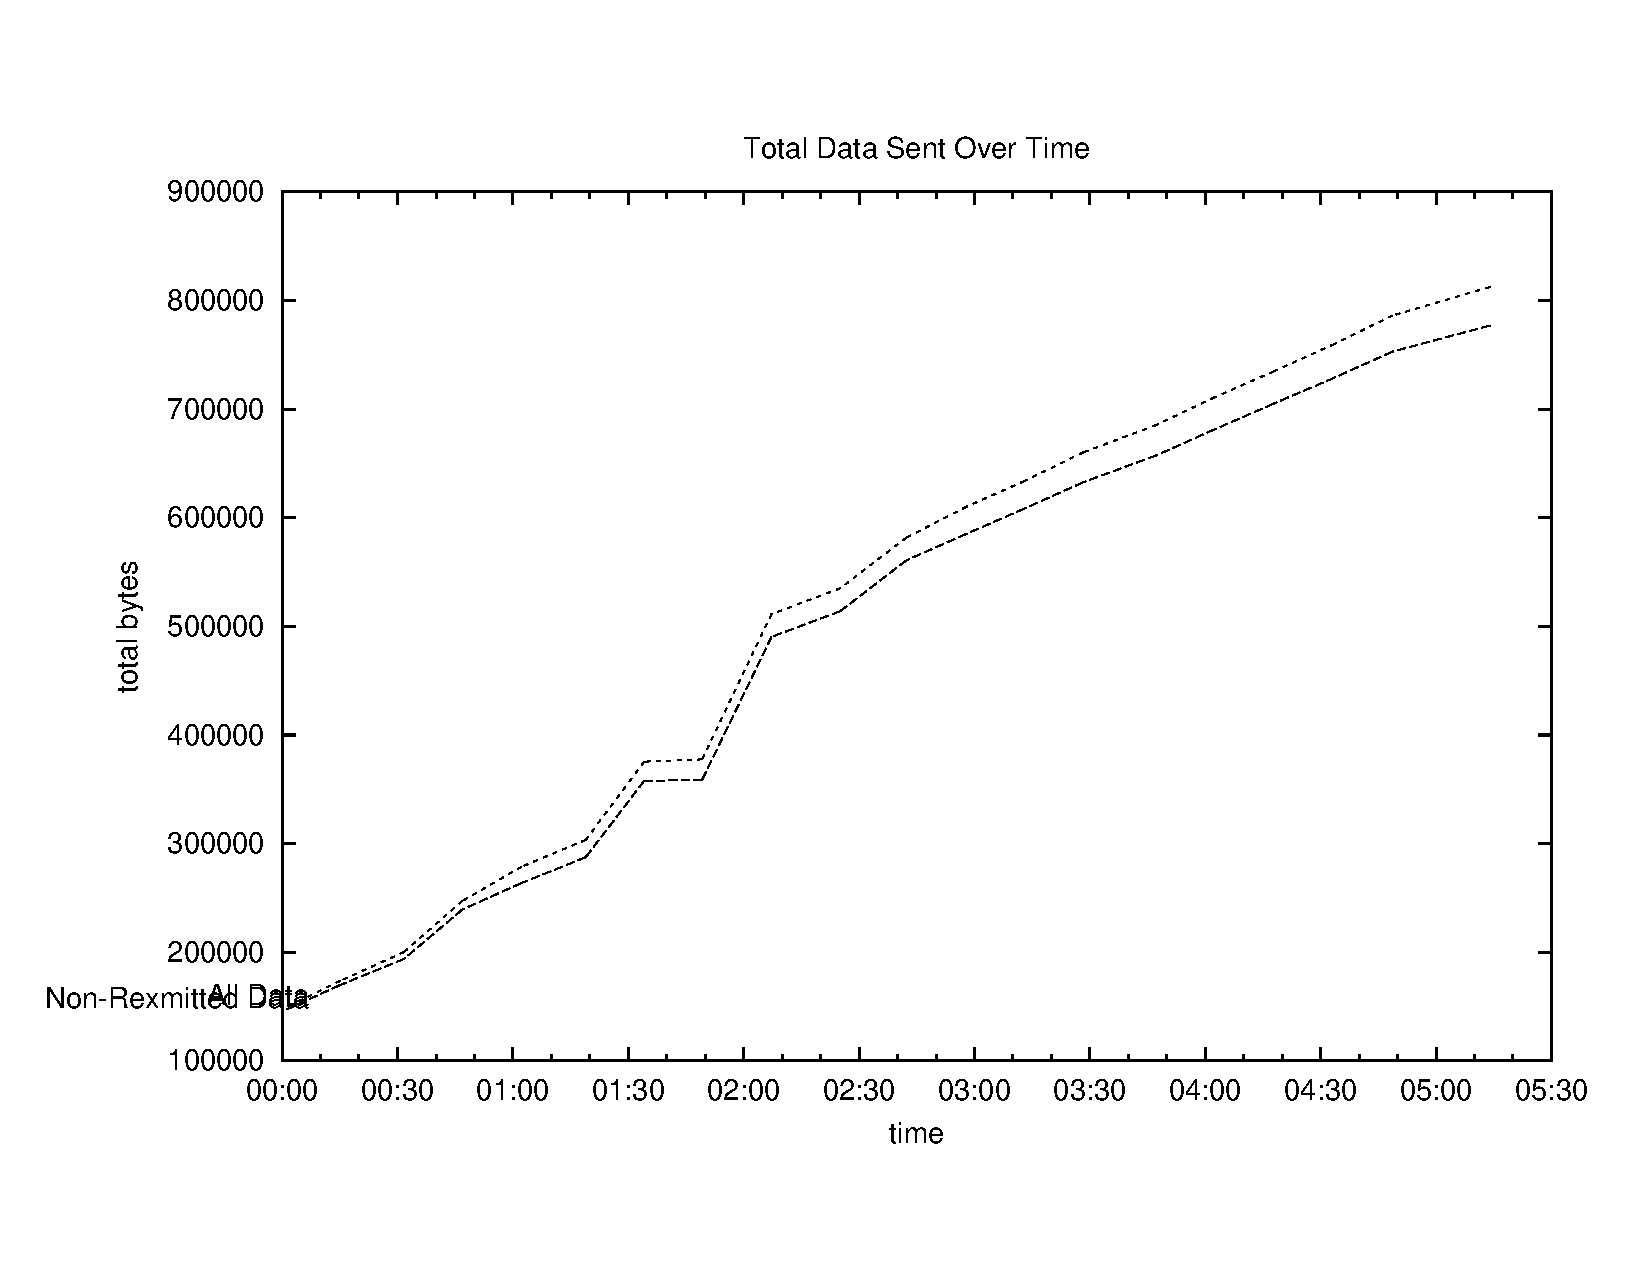
\includegraphics[width=7.2cm]{charts/oneMoreTime_airplay_android}}
\hfill
\subfigure[DLNA]{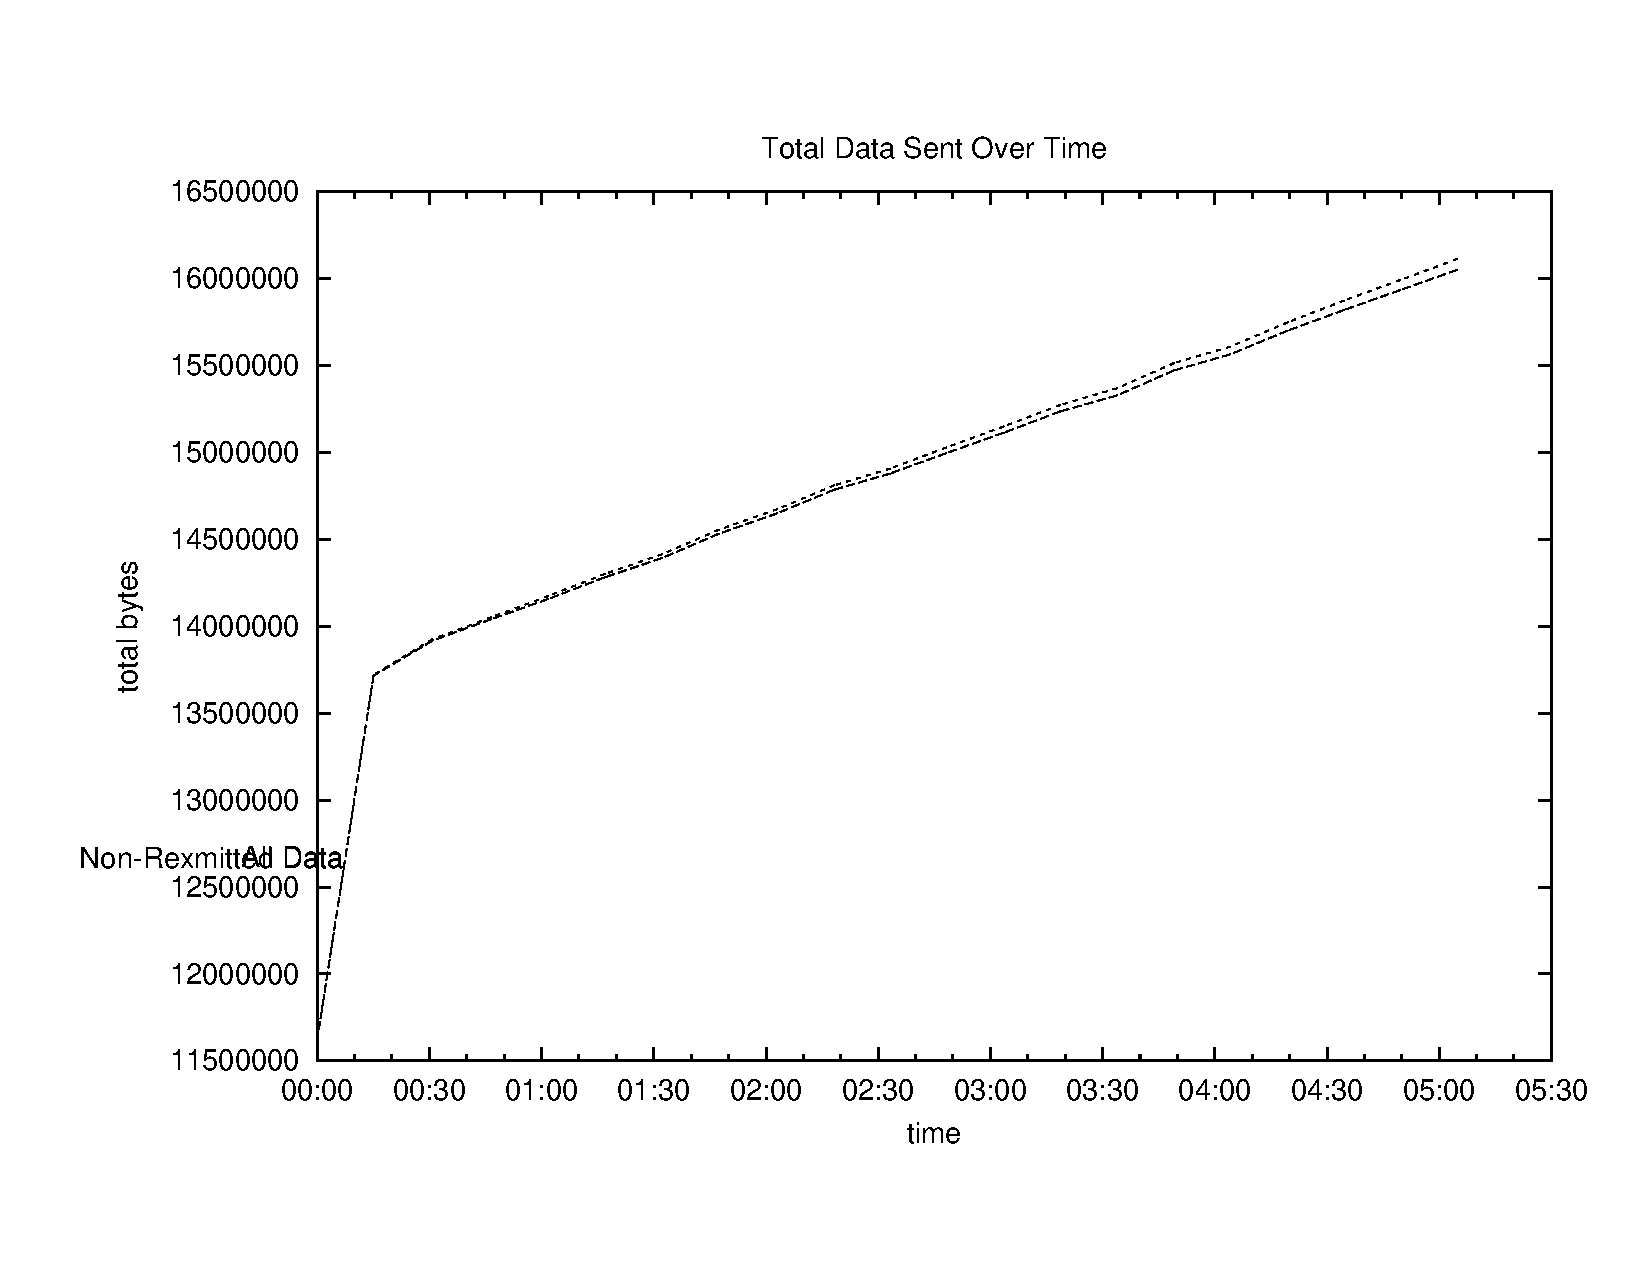
\includegraphics[width=7.2cm]{charts/oneMoreTime_dlna_android}}
\hfill
\caption{AirPlay vs DLNA streaming traffic
comparison \label{airplay_vs_dlna_traffic}}
\end{figure}

According to Figure \ref{airplay_vs_dlna_traffic}, the stream traffic for
AirPlay and DLNA streaming is very different. For AirPlay streaming, the traffic
growth is nearly linear, because the ROAP is a push like process, content can be
streamed in real time. However, for DLNA streaming, HTTP streaming is a pull
like process, the server fetches content from media server, so the content can
be buffered at the top network speed at the beginning of the playback.
Therefore, there is a short download period at the beginning of DLNA's
graph. \\ 
\\
Next, we try to limit the bandwidth and evaluate the performance change using
two solutions. We limited the bandwidth to 500kbps, 700kbps and 1000kbps
respectively and got Figure \ref{dlna_traffic_bw}:\\

\begin{figure}
\hfill
\subfigure[No
limit]{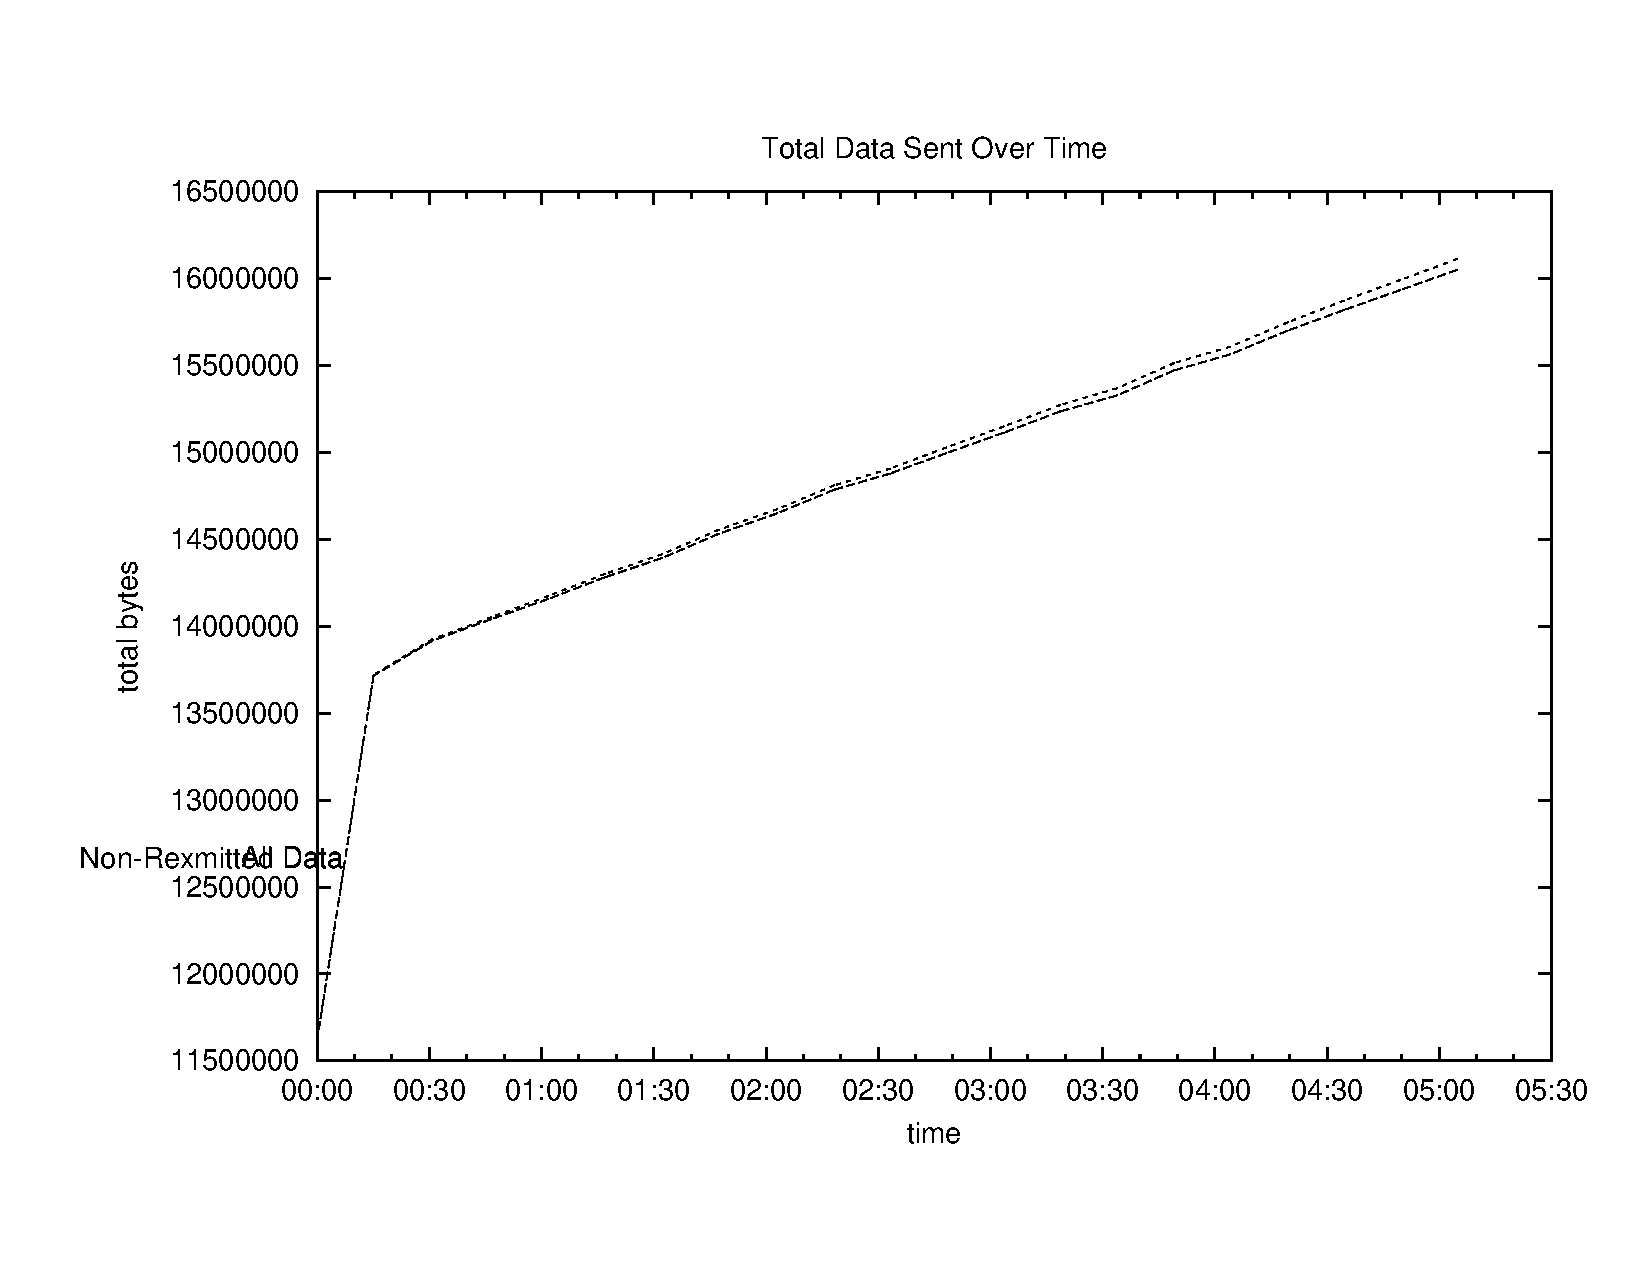
\includegraphics[width=7.2cm]{charts/oneMoreTime_dlna_android}}
\hfill
\subfigure[500kbps]{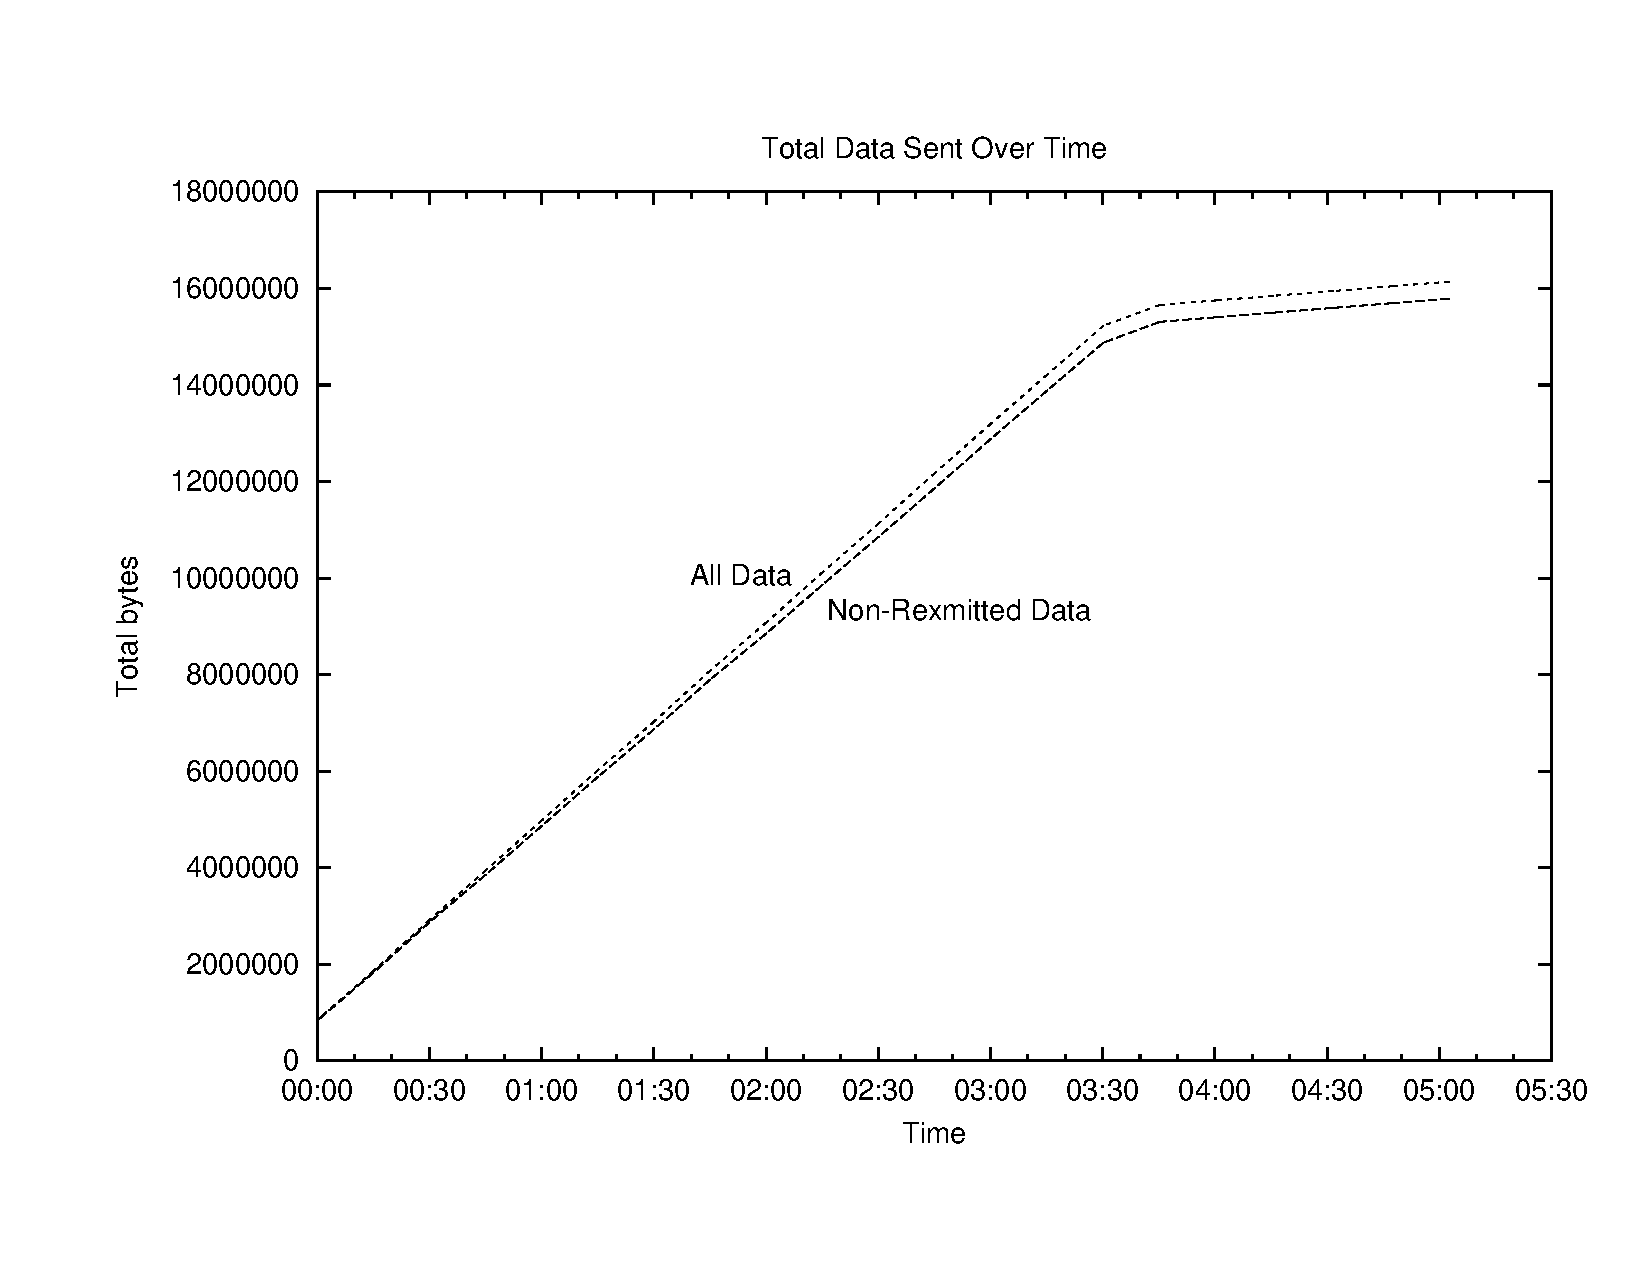
\includegraphics[width=7.2cm]{charts/oneMoreTime_dlna_android_bw_500k}}
\hfill
\subfigure[700kbps]{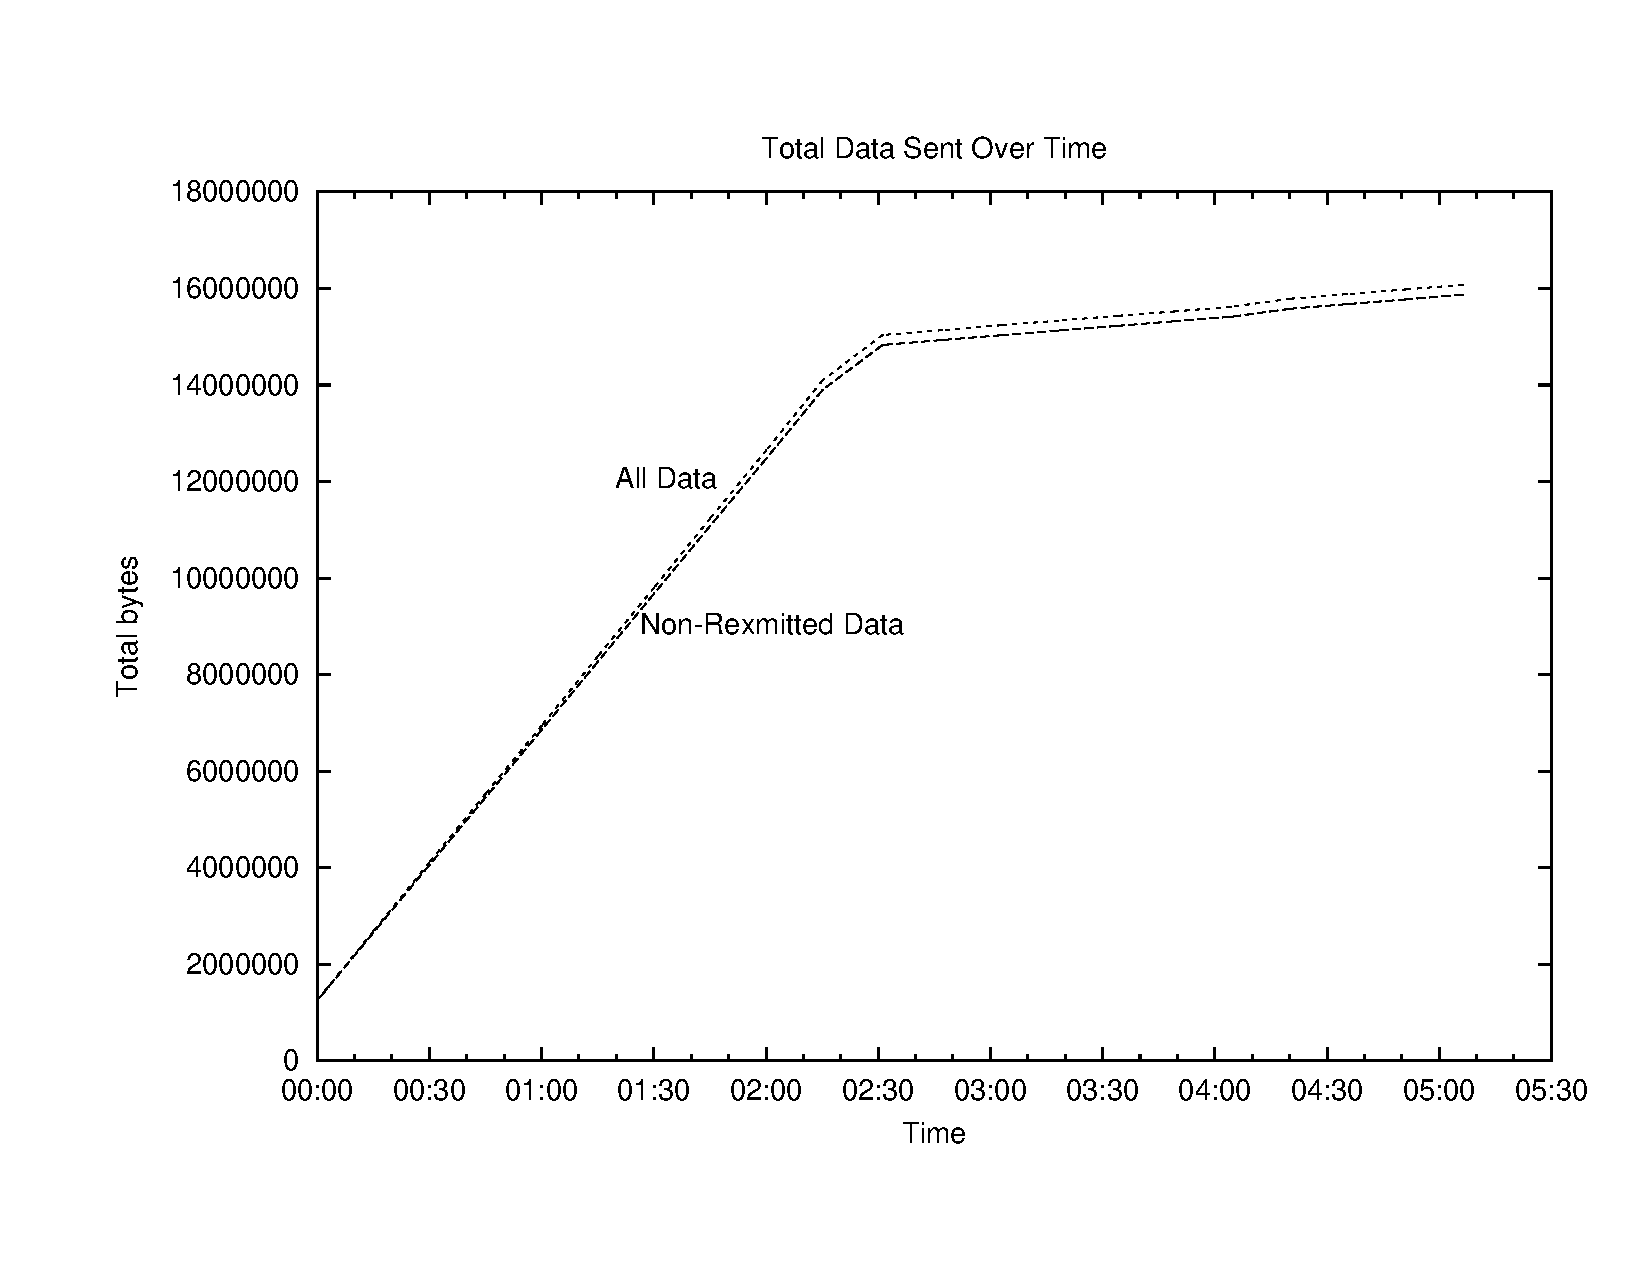
\includegraphics[width=7.2cm]{charts/oneMoreTime_dlna_android_bw_700k}}
\hfill
\subfigure[1000kbps]{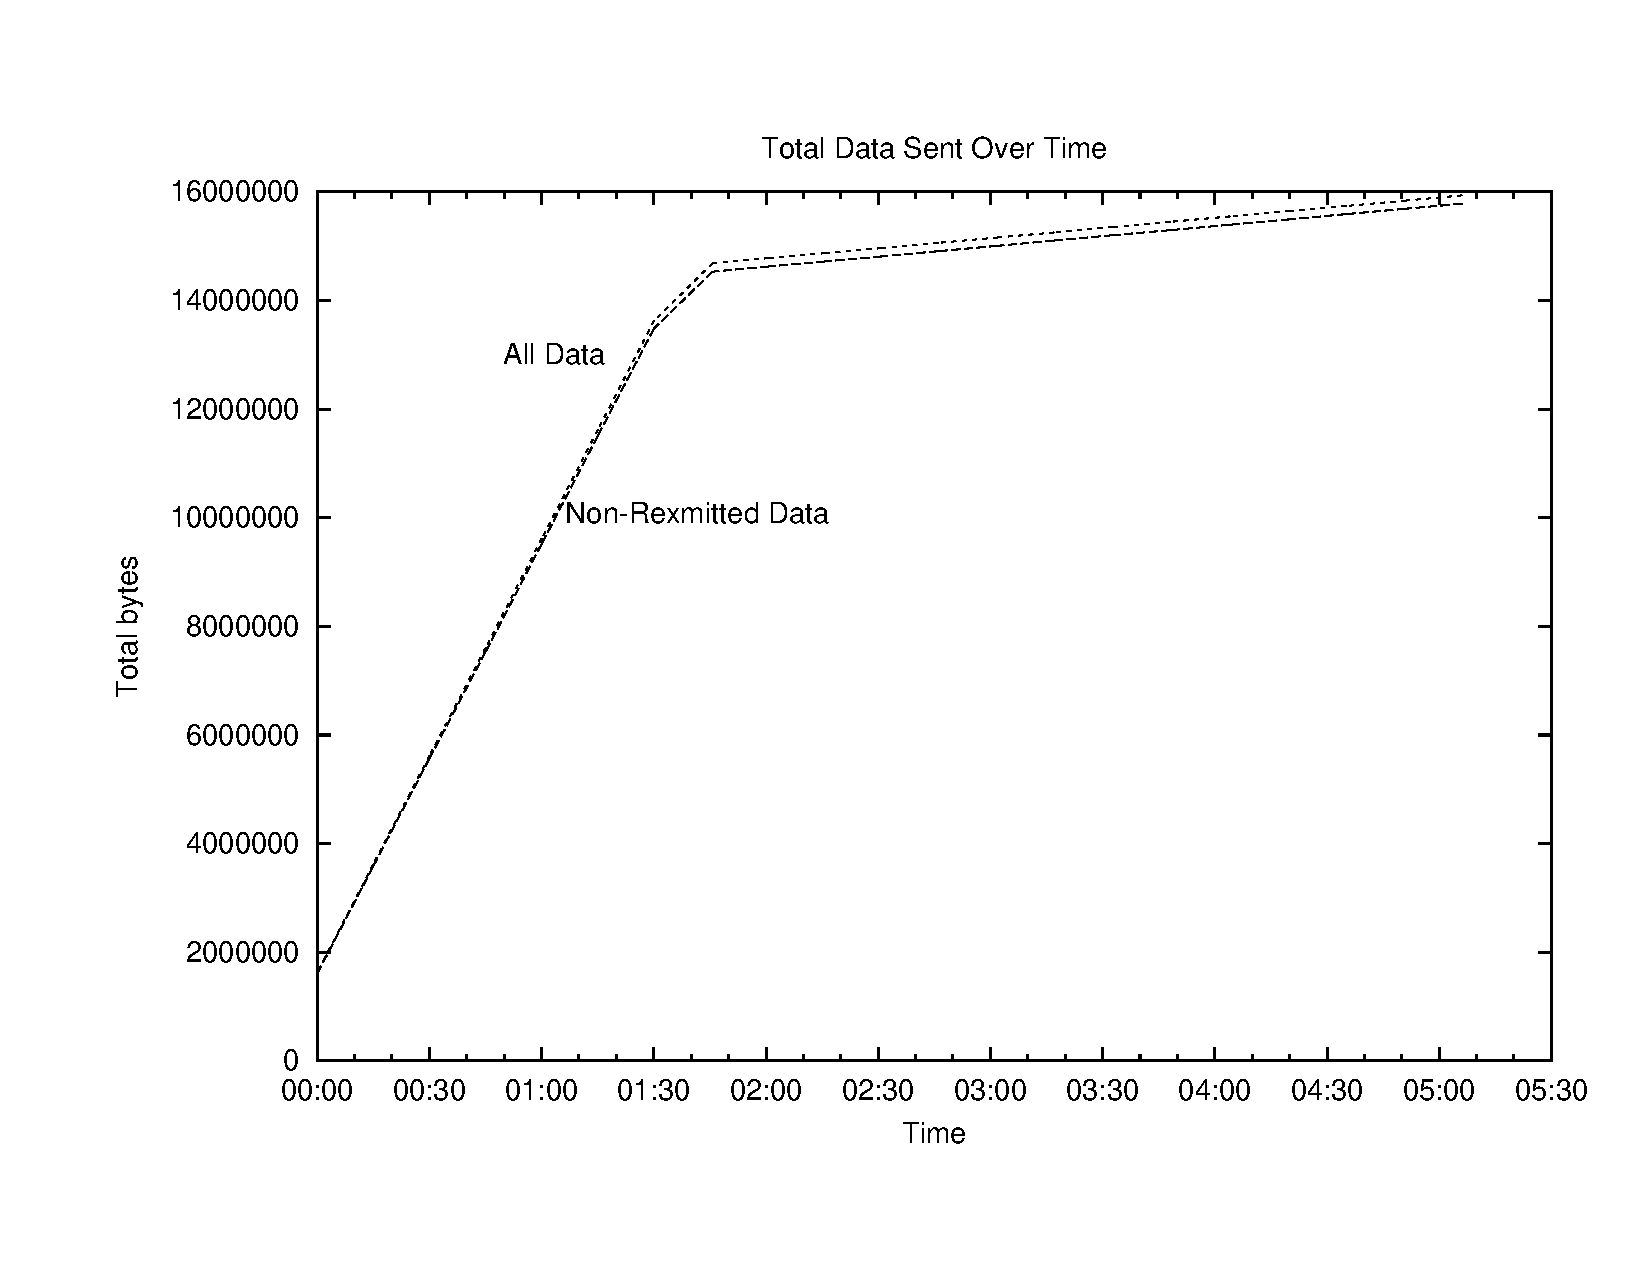
\includegraphics[width=7.2cm]{charts/oneMoreTime_dlna_android_bw_1000k}}
\hfill
\caption{DLNA streaming traffic comparison in
bandwidth constrained situation\label{dlna_traffic_bw}}
\end{figure}


\begin{figure}
\hfill
\subfigure[No
limit]{\includegraphics[width=7.2cm]{charts/AirPlay_traffic_data}}
\hfill
\subfigure[5
percent loss]{\includegraphics[width=7.2cm]{charts/AirPlay_traffic_5loss_data}}
\hfill
\subfigure[10
percent loss]{\includegraphics[width=7.2cm]{charts/AirPlay_traffic_10loss_data}}
\hfill
\subfigure[15
percent loss]{\includegraphics[width=7.2cm]{charts/AirPlay_traffic_15loss_data}}
\hfill
\caption{AirPlay streaming performance in terms of packet loss \label{multiavp}}
\end{figure}


\begin{figure}
\hfill
\subfigure[No
limit]{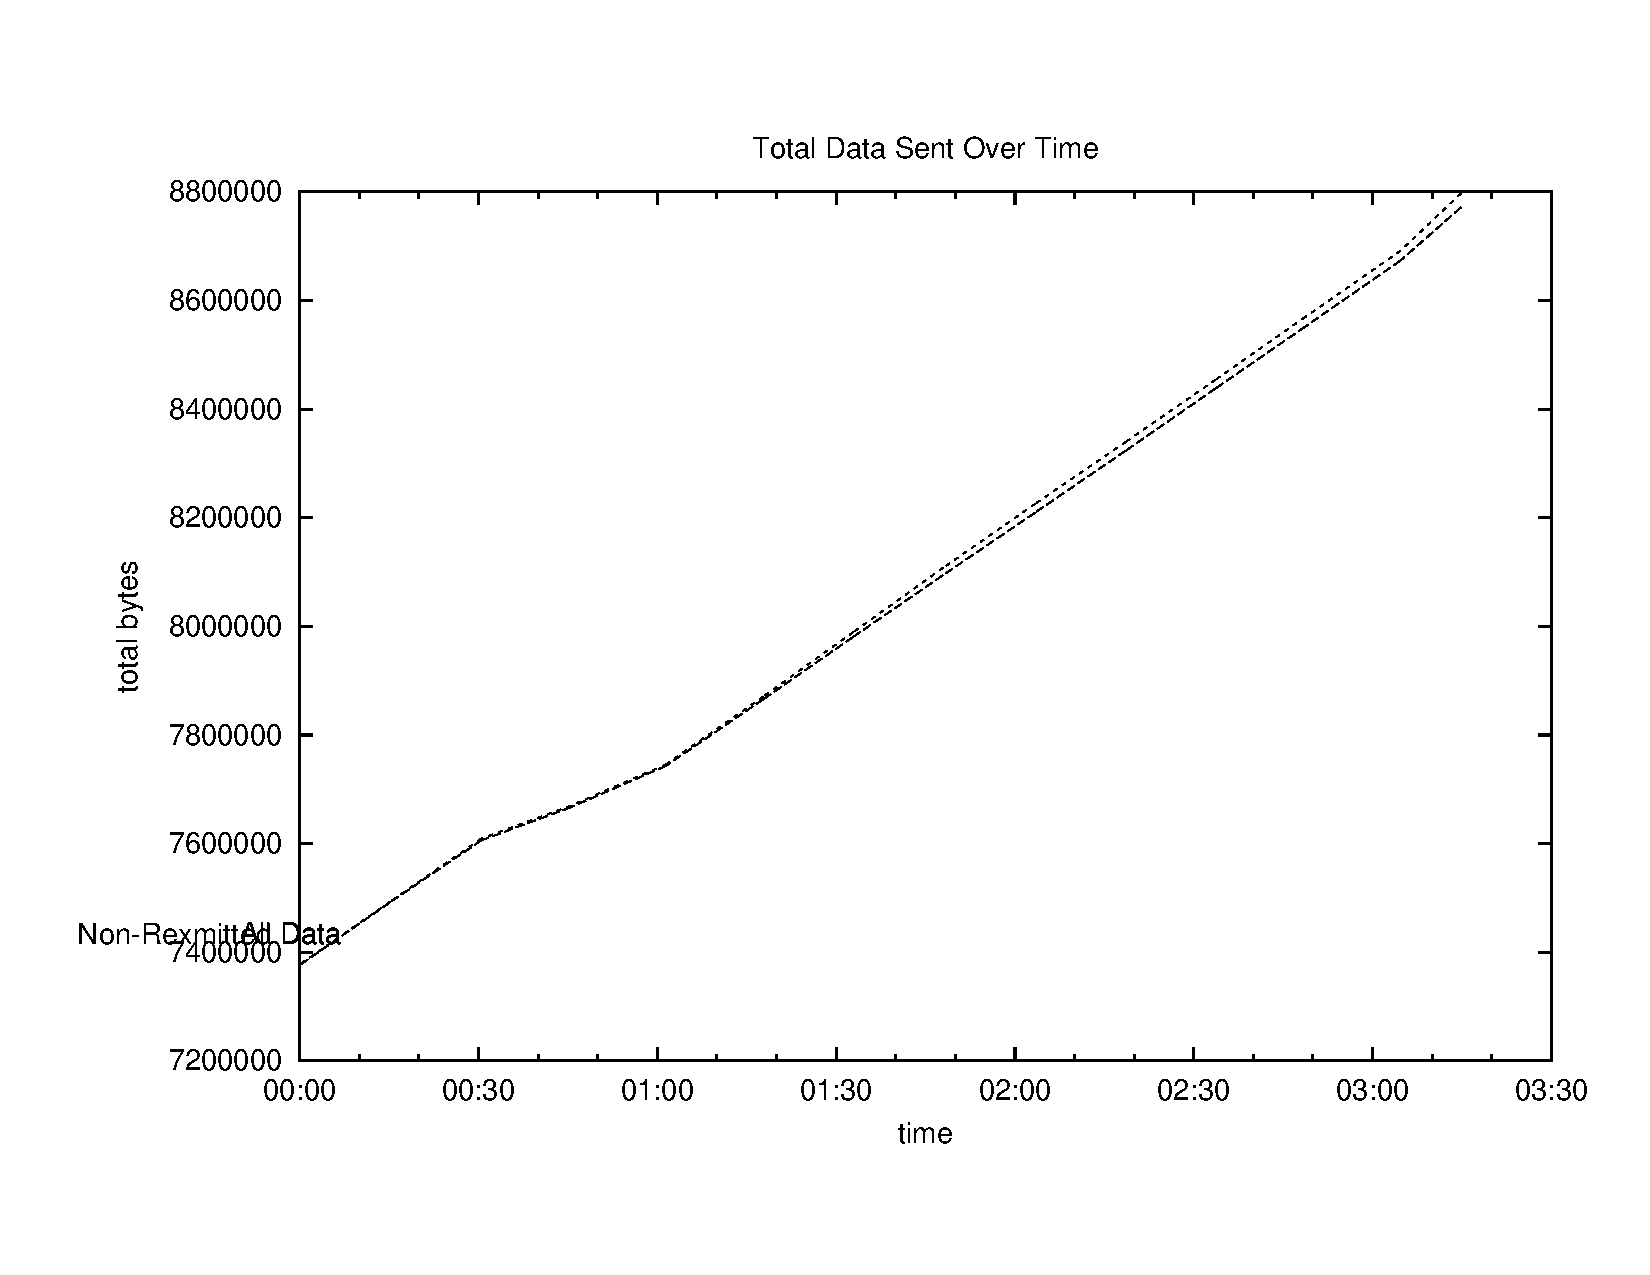
\includegraphics[width=7.2cm]{charts/dlna_traffic_data}}
\hfill
\subfigure[5
percent loss]{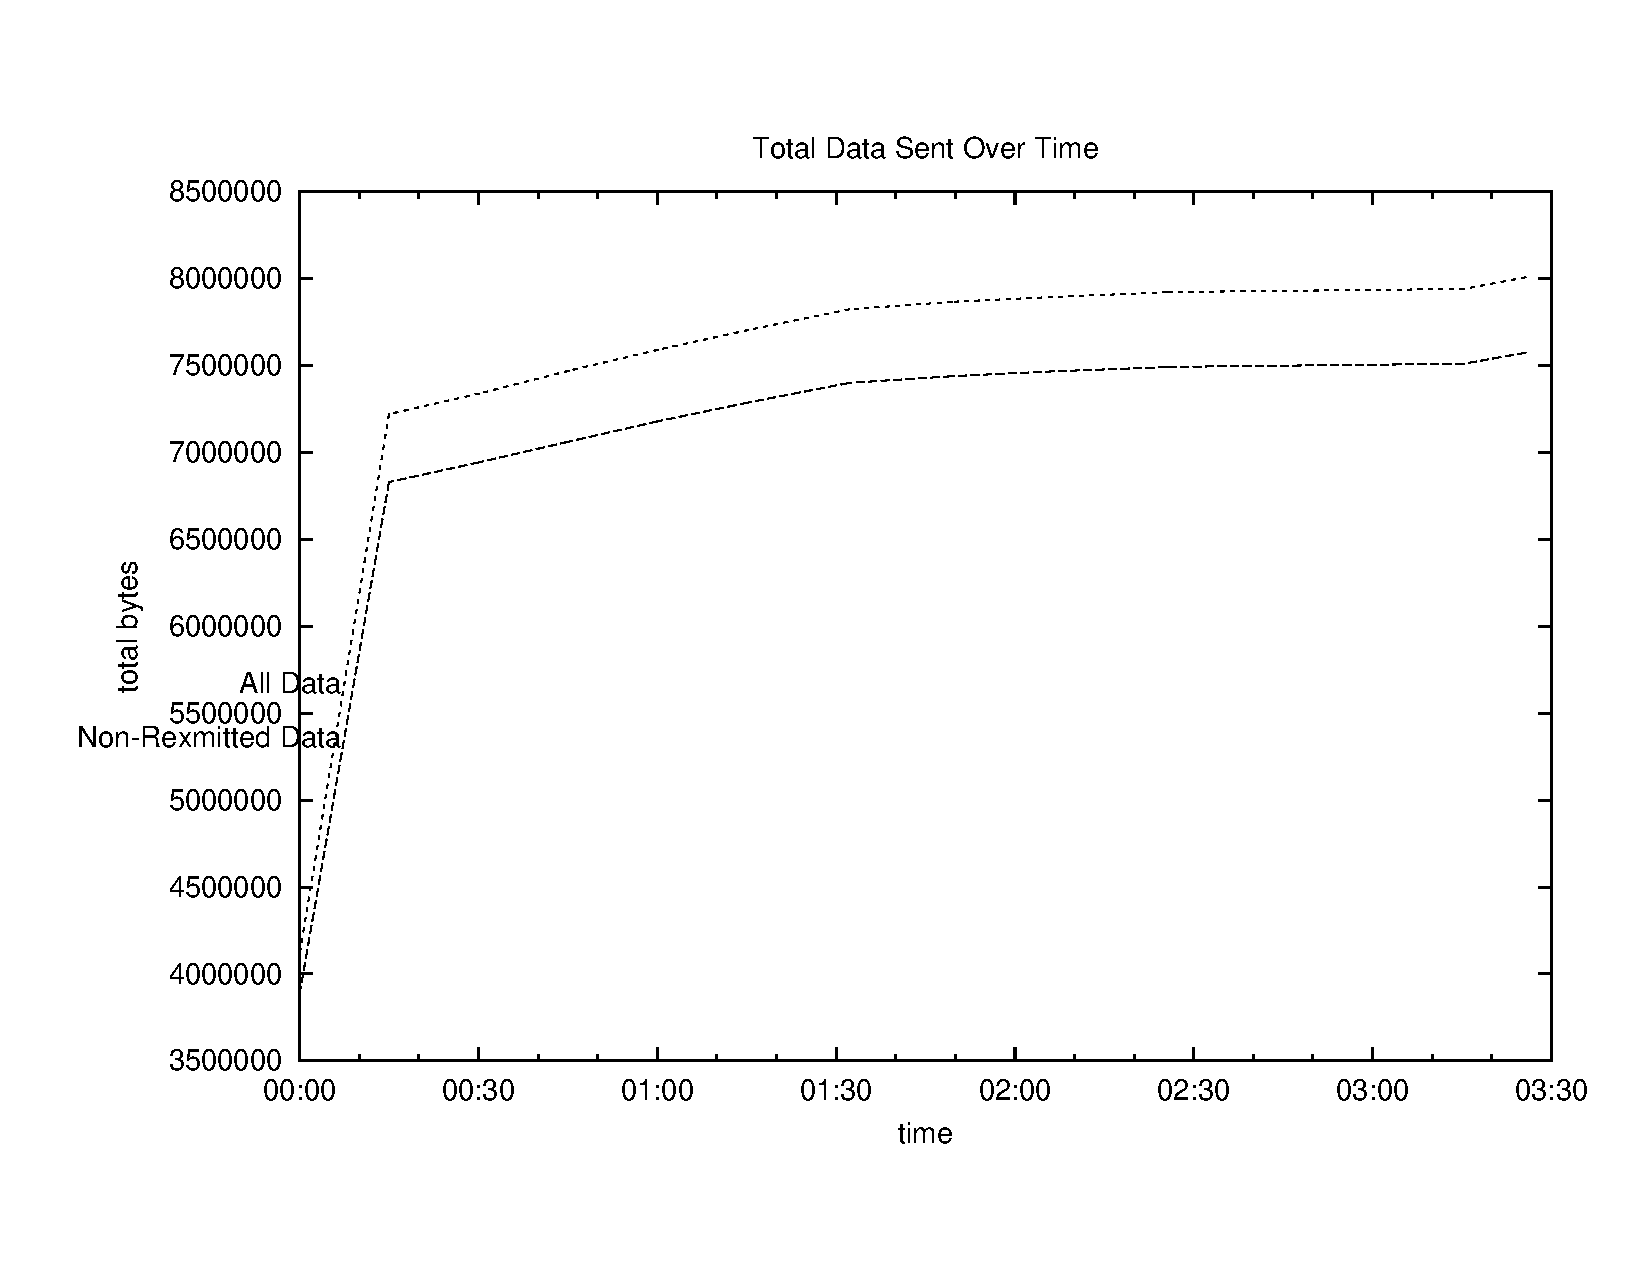
\includegraphics[width=7.2cm]{charts/dlna_traffic_5loss_data}}
\hfill
\subfigure[10
percent loss]{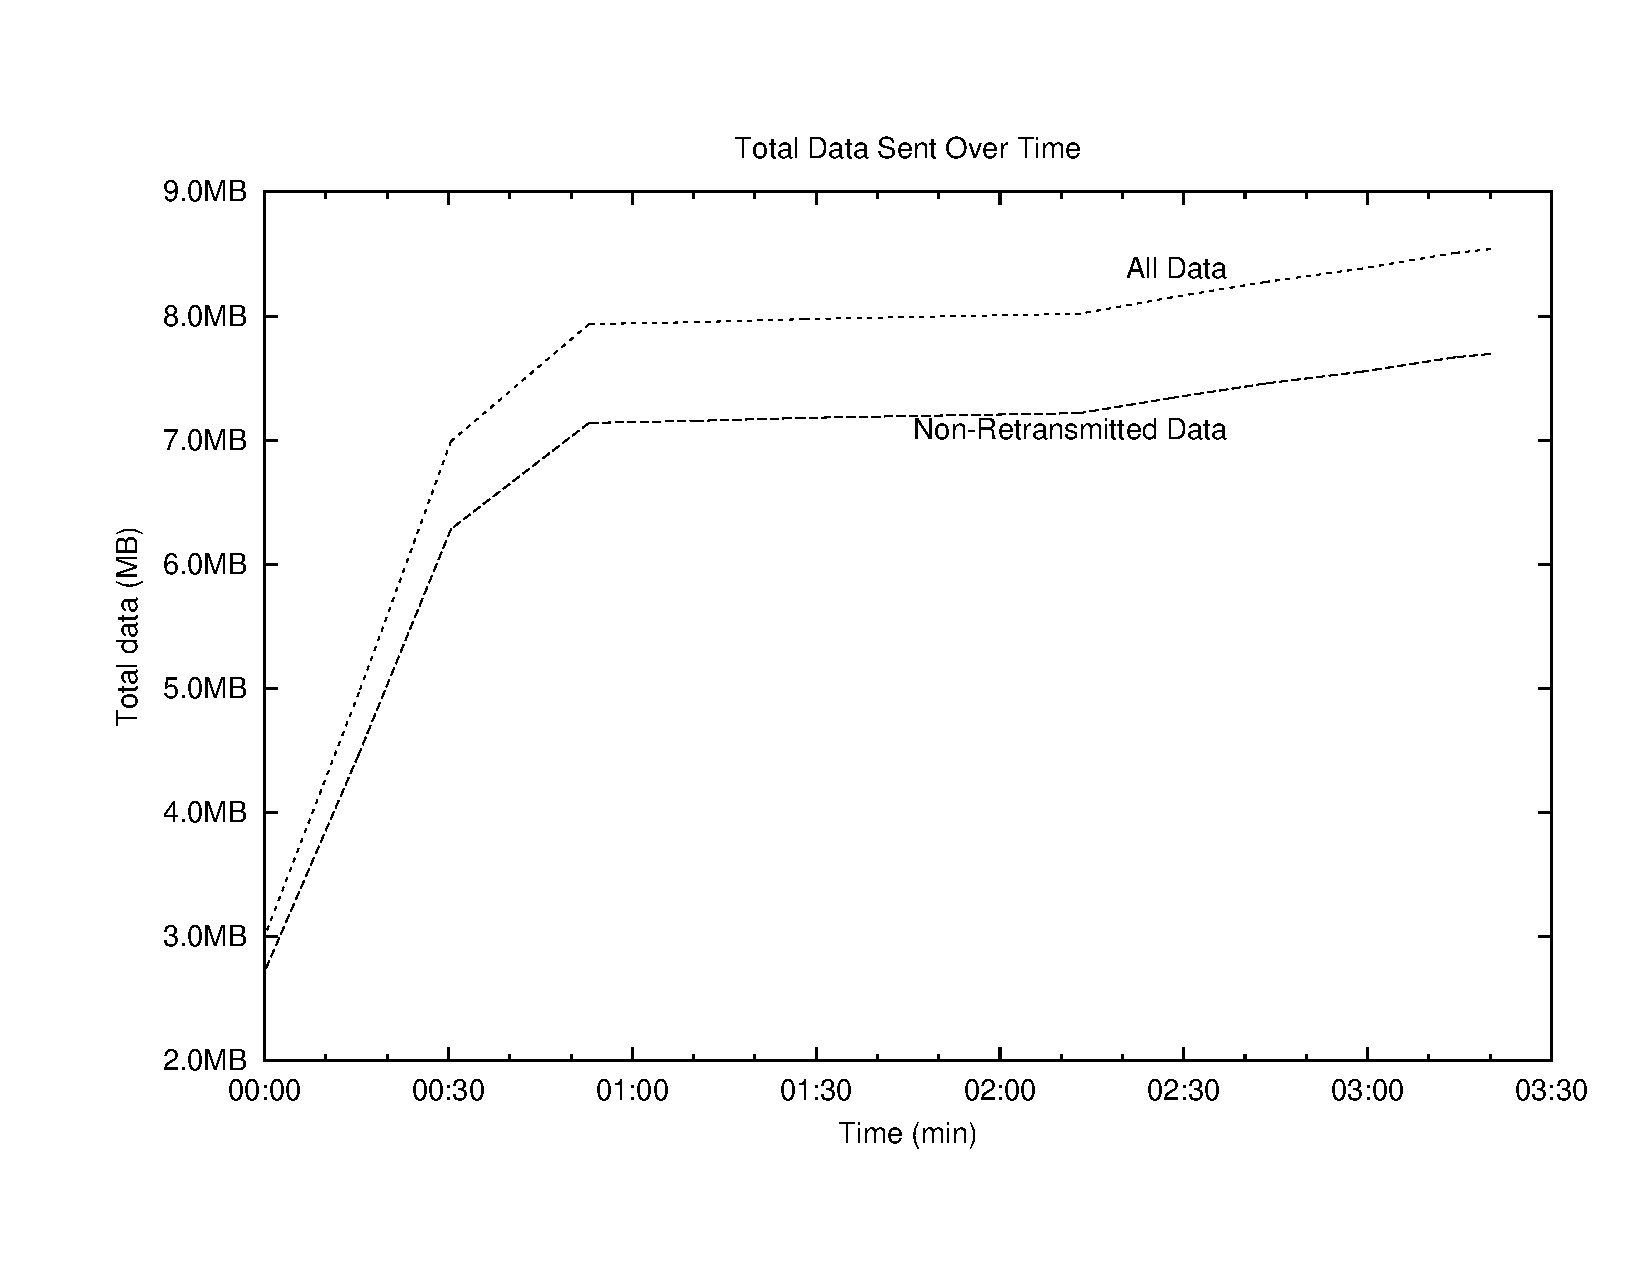
\includegraphics[width=7.2cm]{charts/dlna_traffic_10loss_data}}
\hfill
\subfigure[15
percent loss]{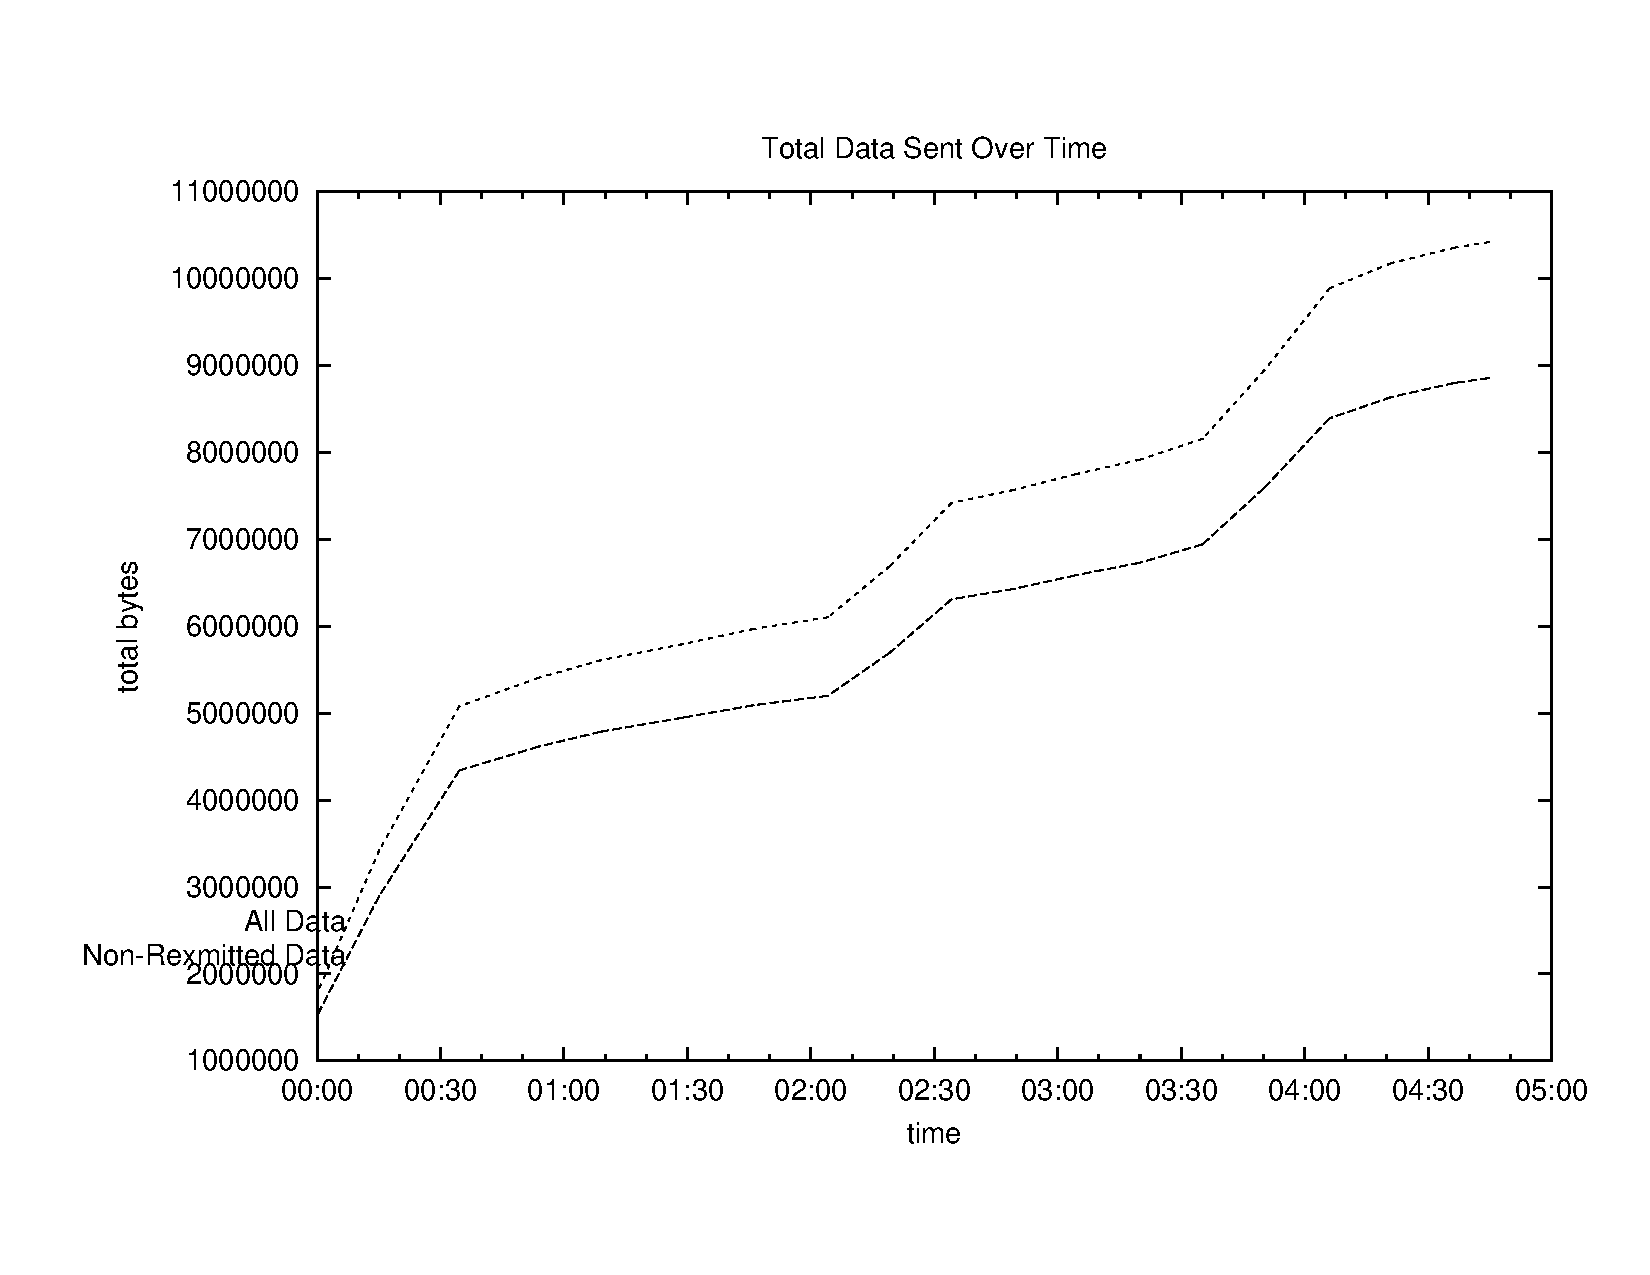
\includegraphics[width=7.2cm]{charts/dlna_traffic_15loss_data}}
\hfill
\caption{DLNA streaming performance in terms of packet loss \label{multiavp}}
\end{figure}



\begin{figure}
\hfill
\subfigure[AirPlay
normal]{\includegraphics[width=7.2cm]{charts/AirPlay_traffic_data}}
\hfill
\subfigure[DLNA normal]{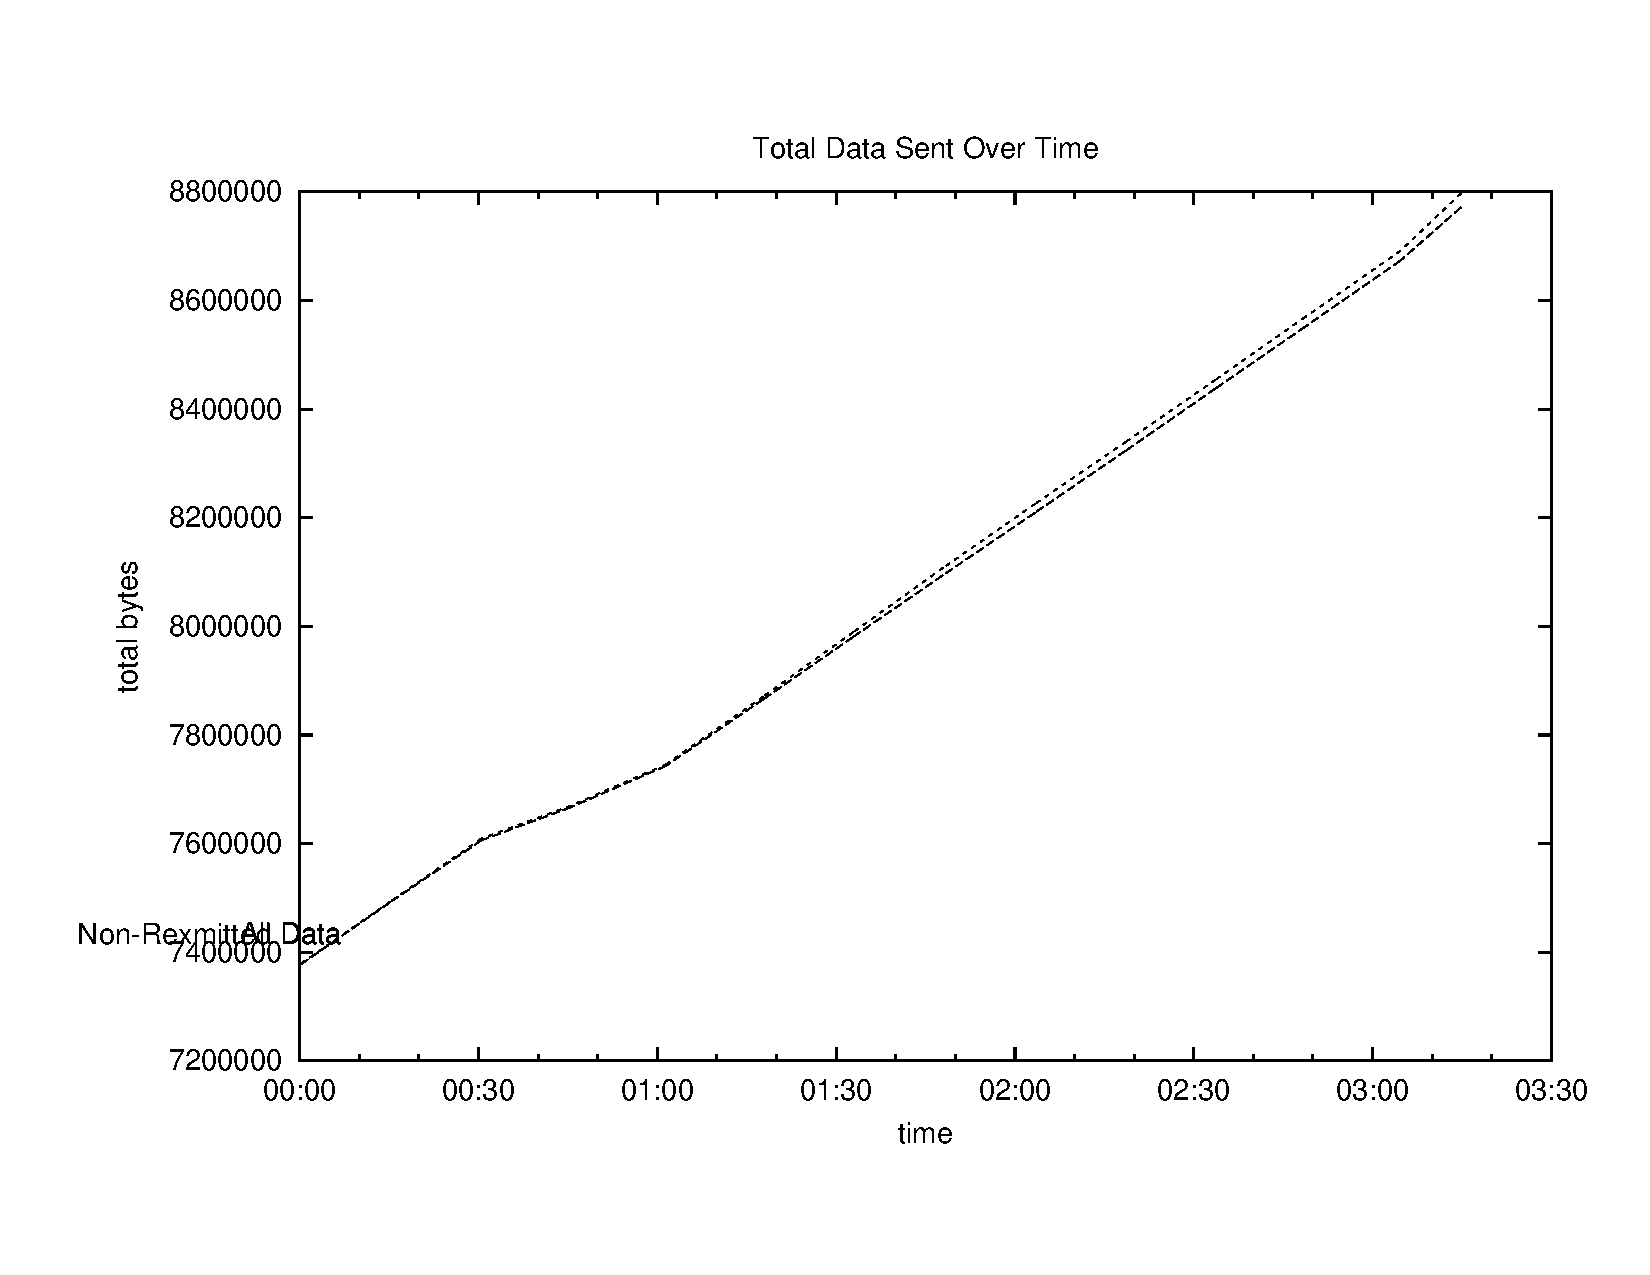
\includegraphics[width=7.2cm]{charts/dlna_traffic_data}}
\hfill
\subfigure[AirPlay
bad
network]{\includegraphics[width=7.2cm]{charts/badnetwork_AirPlay_traffic_data}}
\hfill
\subfigure[DLNA
bad network]{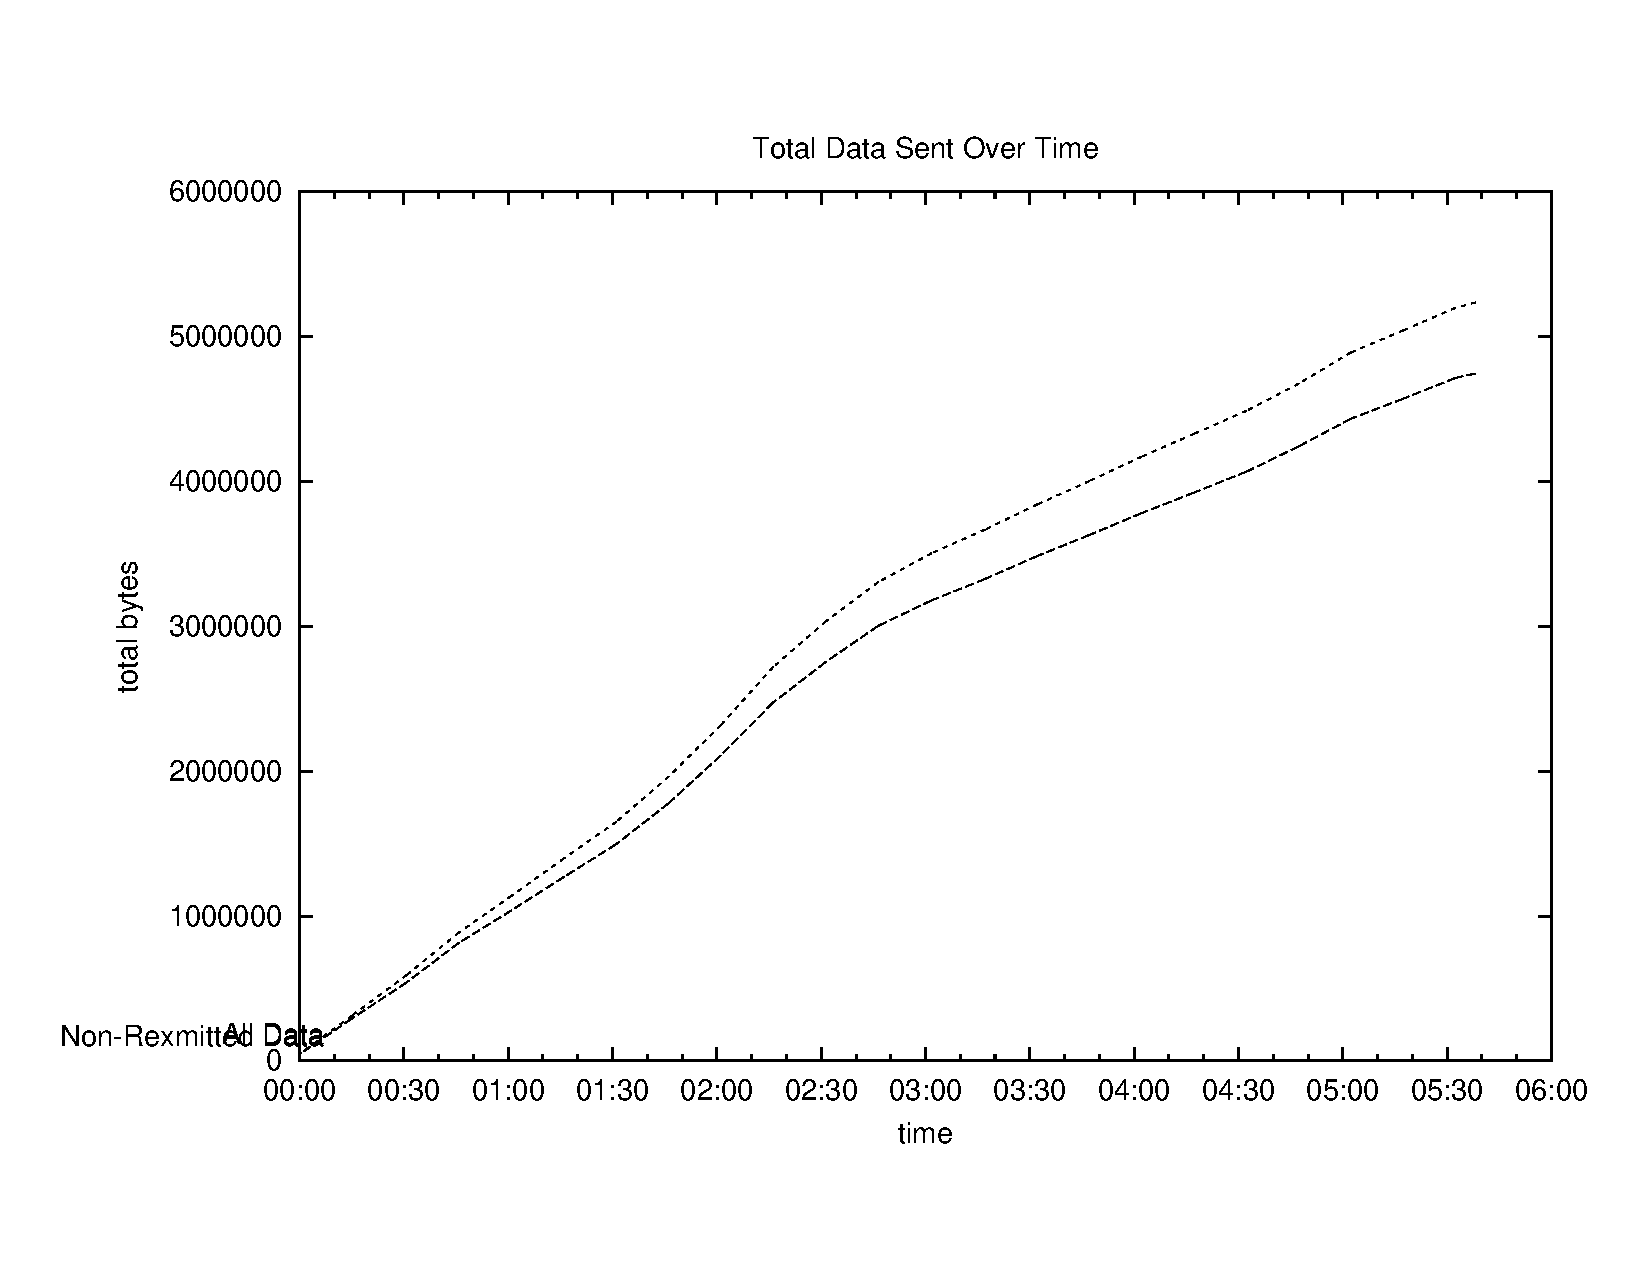
\includegraphics[width=7.2cm]{charts/badnetwork_dlna_traffic_data}}
\hfill
\caption{Comparison of AirPlay and DLNA in bad network conditions
\label{multiavp}}
\end{figure}


\subsection{Statistics}
Through 16 months' releasing, our application have achieved 924000 downloads from 223 countries all around the world, with around 10000 daily active users. This means our users almost cover 99% of the earth, a world map of our users is shown in Figure \ref{user_map}. So far, we got ratings from 10253 users, currently the average rating is 3.9 out of 5. The distribution is shown in Figure \ref{ratings}.

\begin{figure}[htb]
\centering 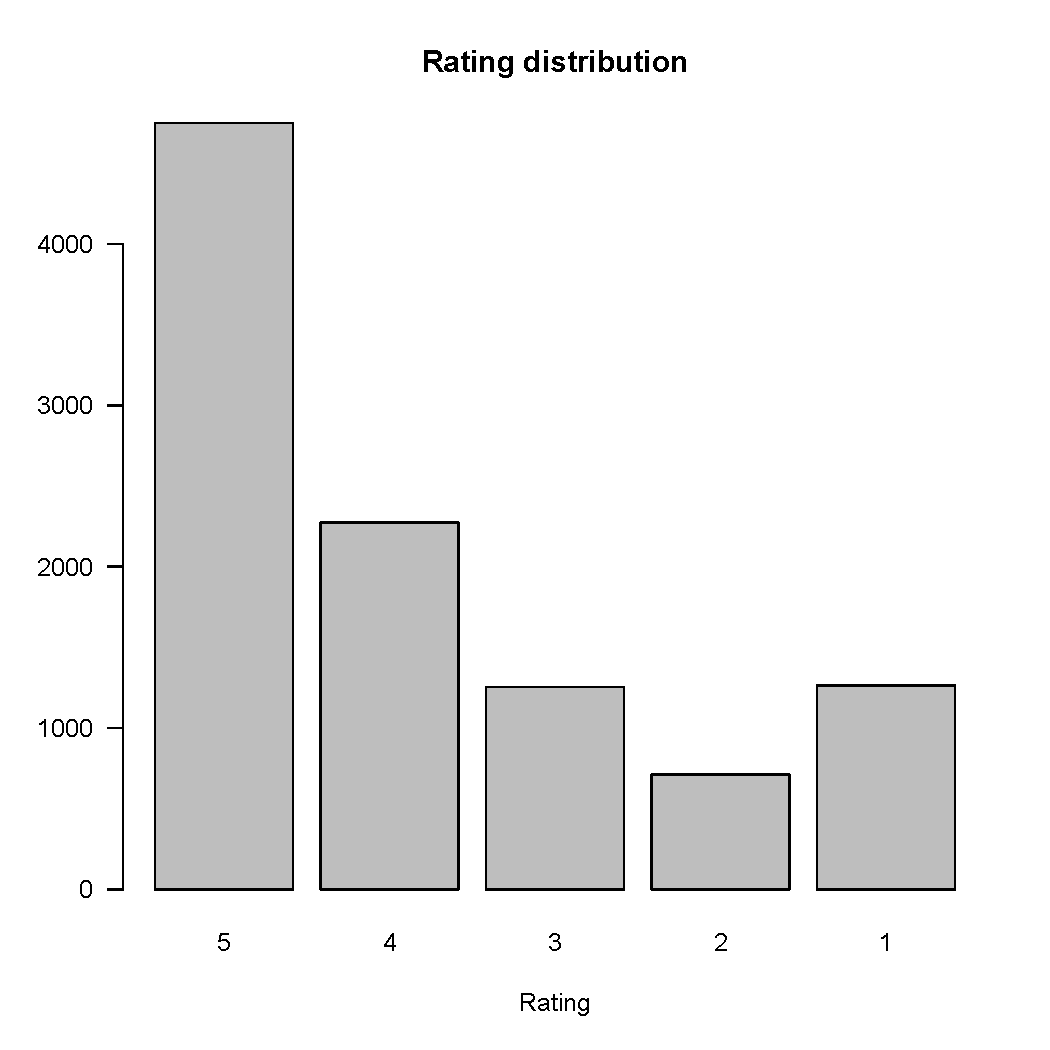
\includegraphics[height=9cm]{charts/rating_distribution}
\caption{Rating distribution\label{ratings}}
\end{figure}

According to the rating distribution graph, most users are satisfied with our solution and gave 5 stars rating. However, the average rating is heavily influenced by the 1 star rating users. The reason of those unsatisfied users is that it happens that the receiver user have in home is not compatible with our application due to different reasons. It might be protocols are not supported yet, such as Roku box. Network condition problem also contributes to the incompatibility problem, some routers have by default disabled multicast due to security reasons. Another major cause of the incompatibility problem is that even use the same protocol, take DLNA for example, a minor implementation difference may cause the break of connection, thus, in the later phase, we have made receiver specific hacks to make our application work with most DLNA receivers regardless of which implementation they use.
In terms of user distribution, in 16 months, our application turns out to be popular in countries like France, United States, Germany, United Kingdom and Brazil. The user distribution is shown in Figure \ref{user_country}.
\begin{figure}[htb]
\centering 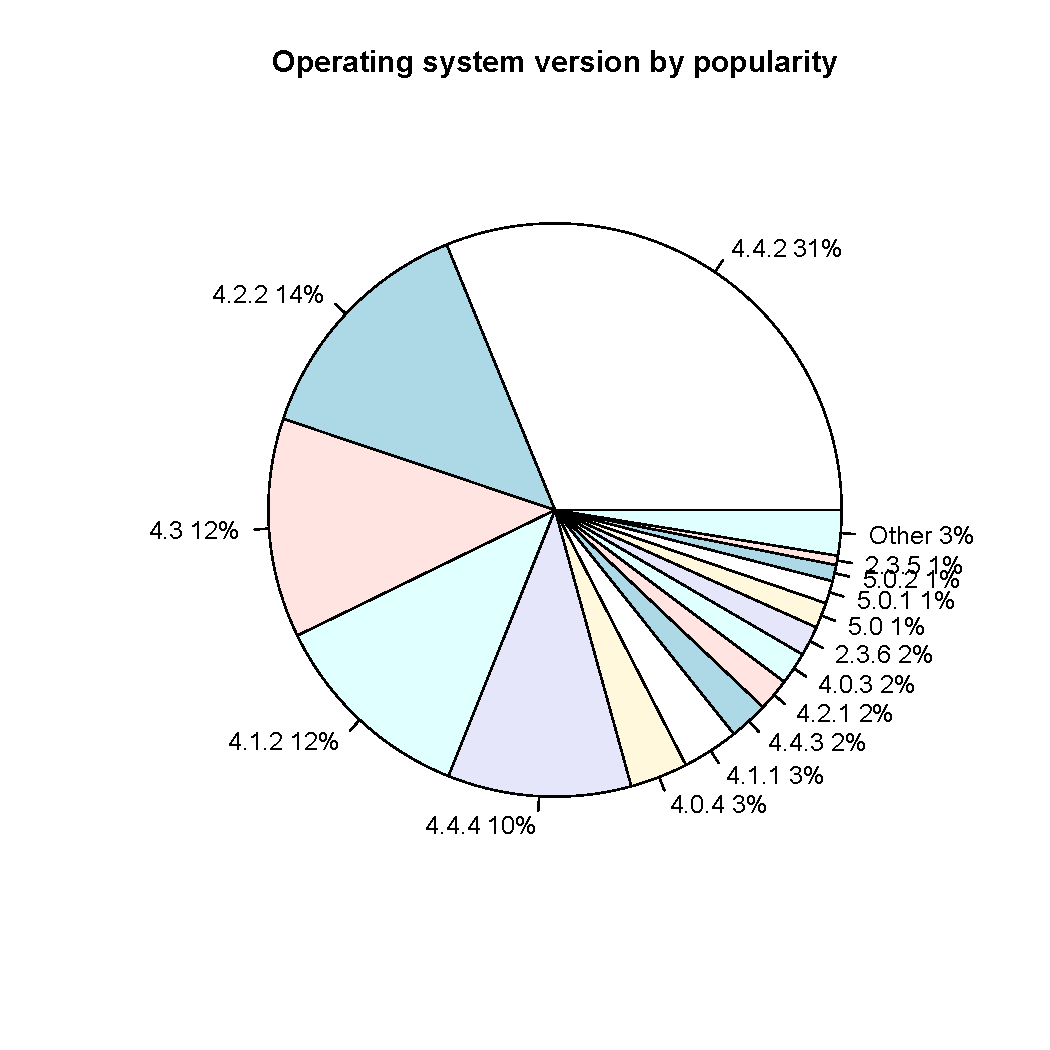
\includegraphics[height=9cm]{charts/os_version_popularity}
\caption{Popularity of different Android versions \label{os_versions}}
\end{figure}

\begin{figure}[htb]
\centering 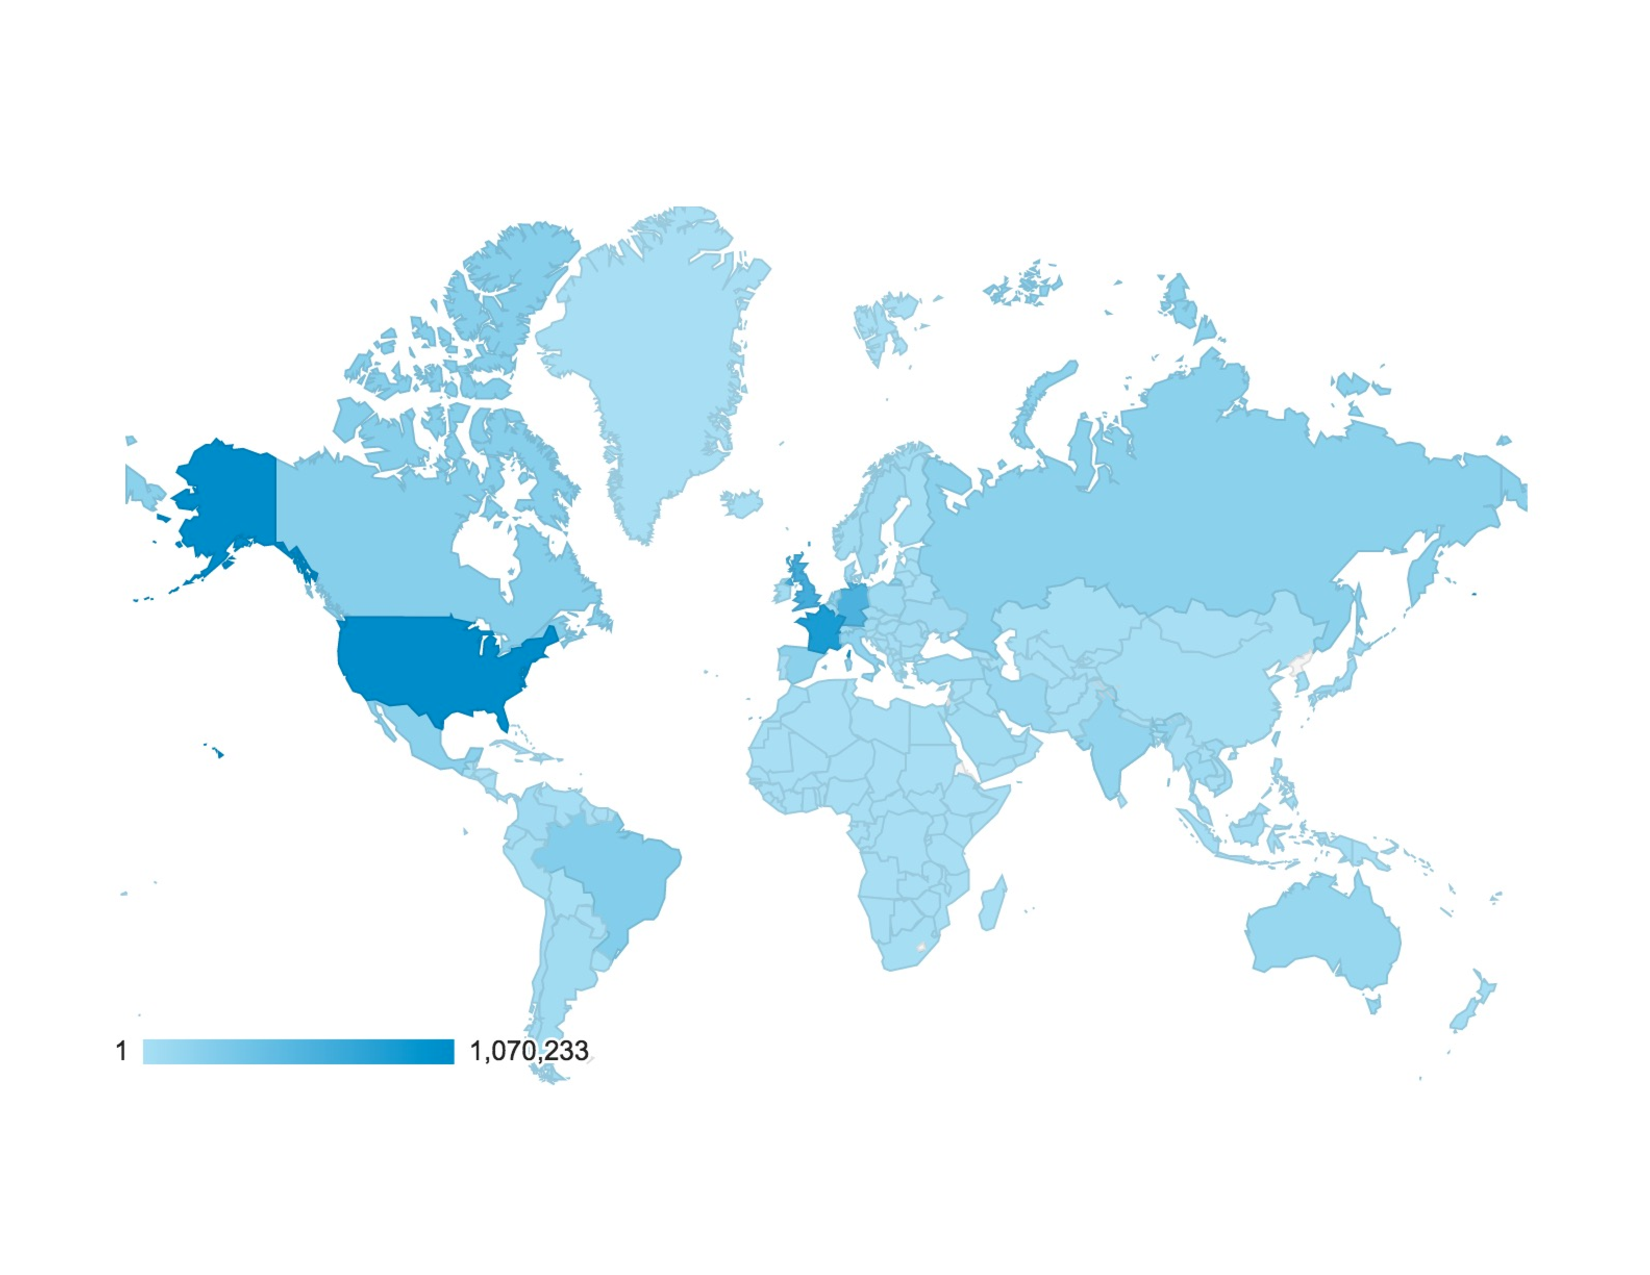
\includegraphics[width=14cm]{charts/session_world_map}
\caption{World map of visits \label{user_map}}
\end{figure}

\begin{figure}[htb]
\centering 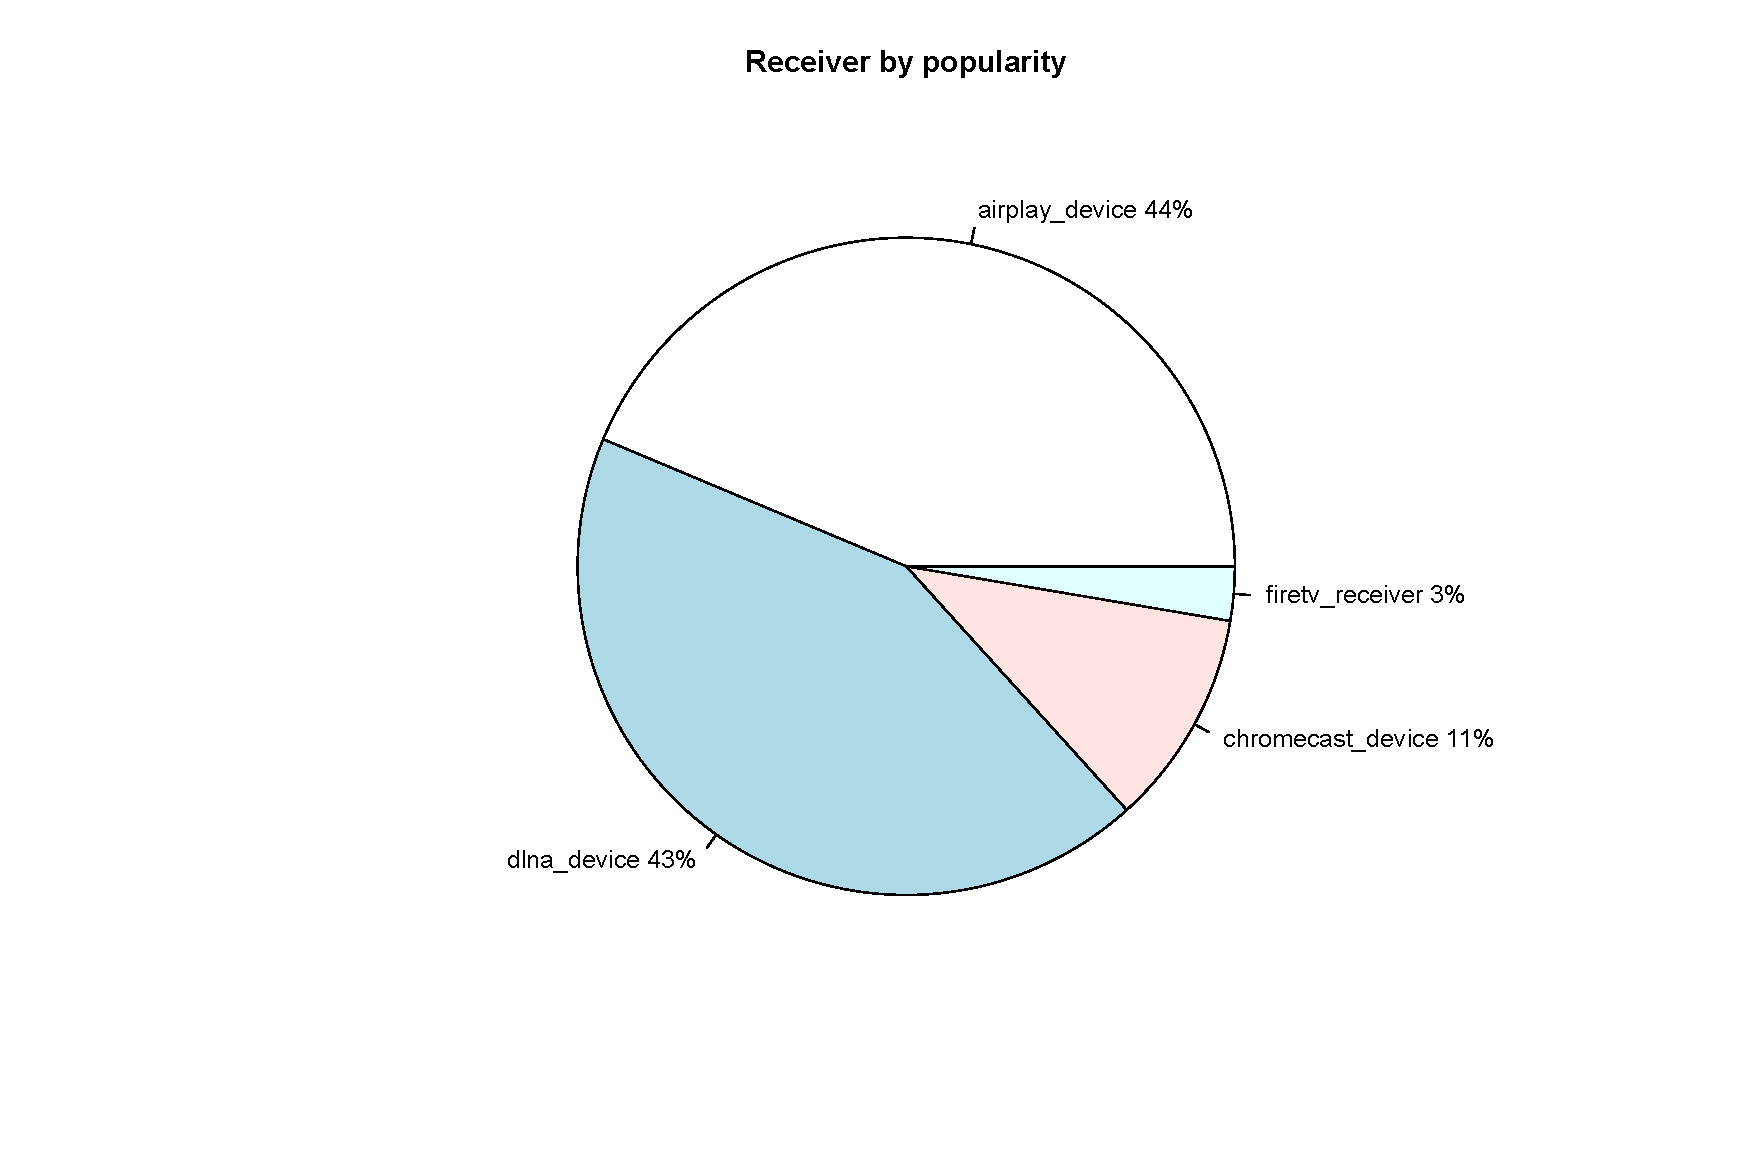
\includegraphics[height=9cm]{charts/receiver_popularity}
\caption{Popularity of receiver types \label{receiver_types}}
\end{figure}

\begin{figure}[htb]
\centering 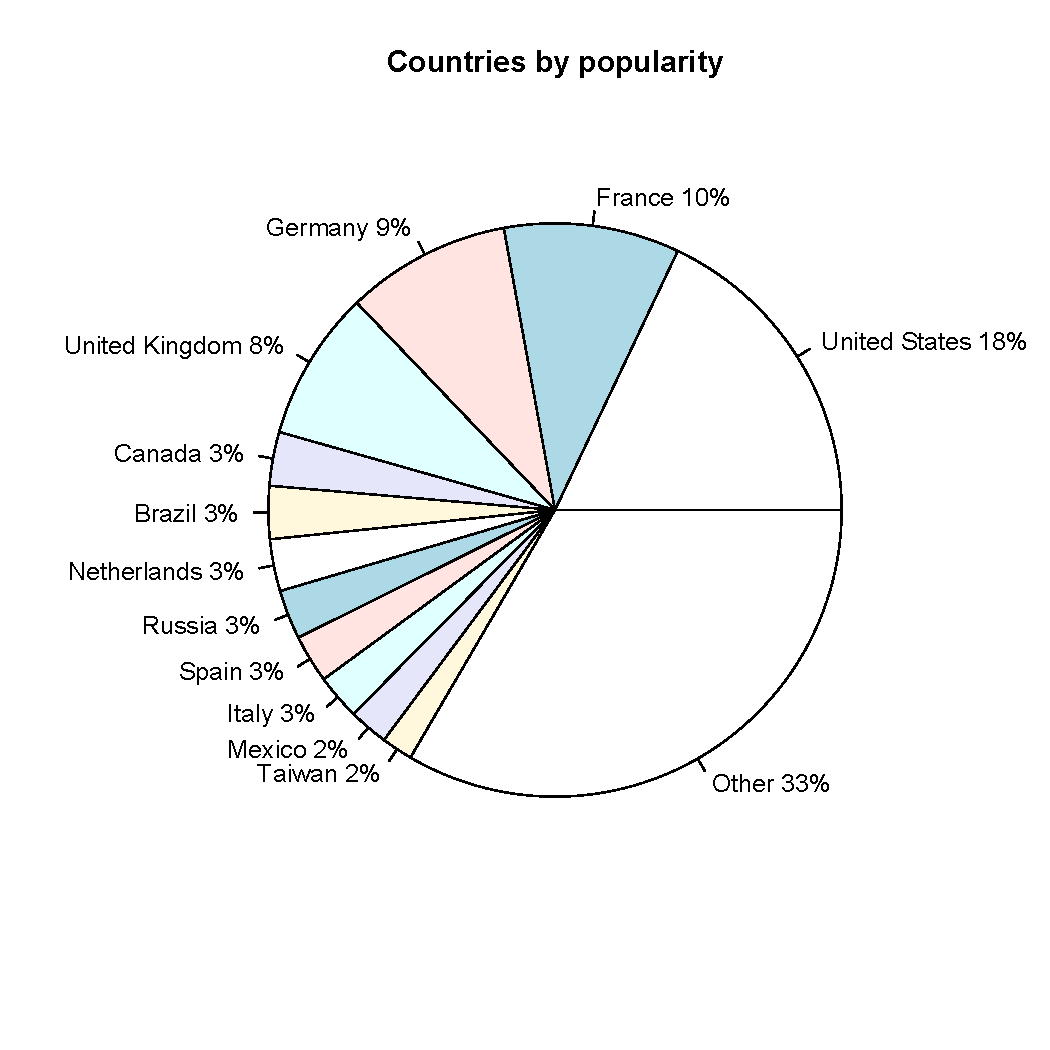
\includegraphics[height=9cm]{charts/country_popularity}
\caption{Popularity in different countries \label{user_country}}
\end{figure}


\begin{figure}[htb]
\centering 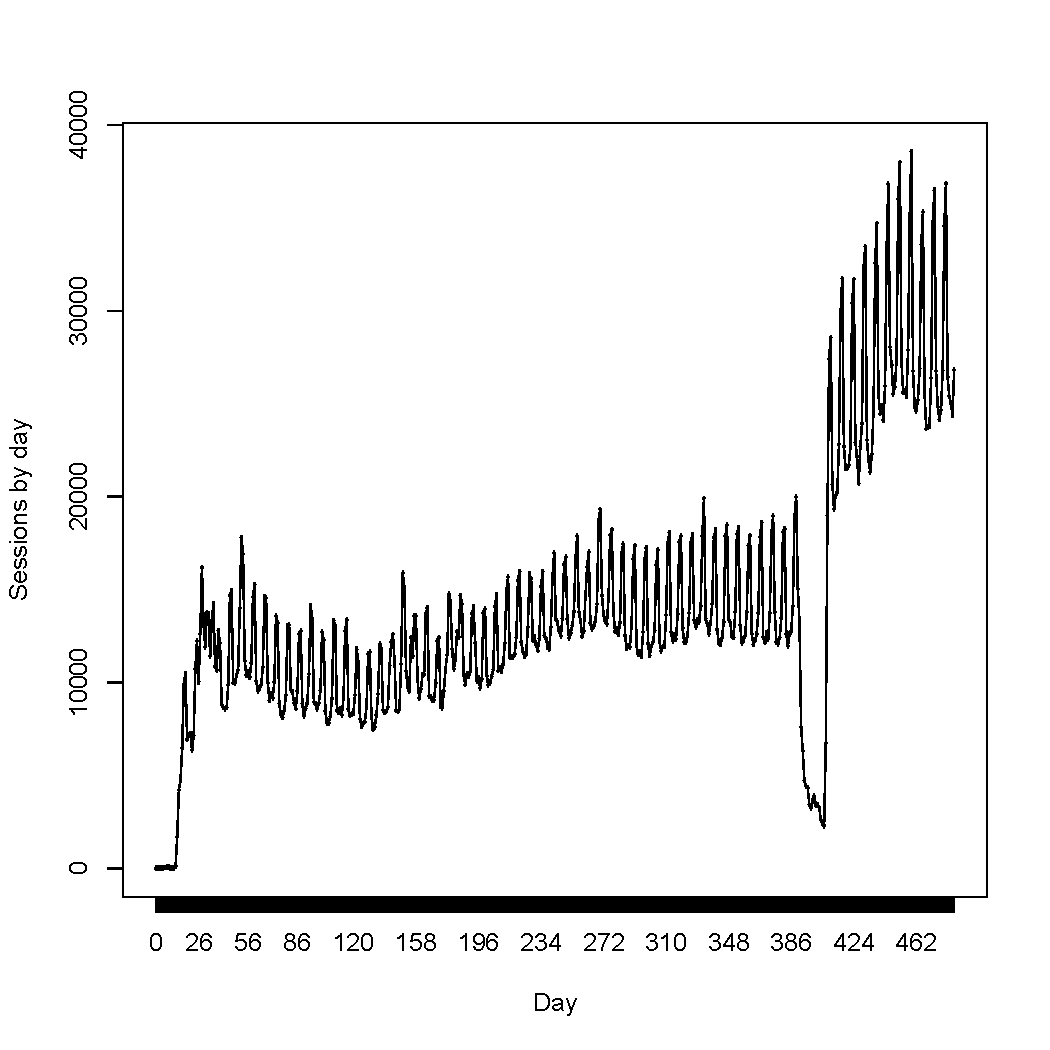
\includegraphics[height=9cm]{charts/sessions_per_day}
\caption{Sessions per day \label{sessions_perday}}
\end{figure}

\subsection{User study}
\begin{itemize}
\item[--]What information we can get back from users
\item[--]User behavior/ statistics
\item[--]Improve the application accordingly
\item[--]Strategies for decision making
\end{itemize}
Write result here.